% !TEX root = ../dkilleffer-thesis-proposal.tex
%
\chapter{Prior Work}
\label{sec:priorwork}

%\cleanchapterquote{A picture is worth a thousand words. An interface is worth a thousand pictures.}{Ben Shneiderman}{(Professor for Computer Science)}

%\Blindtext[2][1]

The idea of annotating videos is not entirely new or novel, but such tools have not become commonplace in the same way that high quality image editing software and facial recognition algorithms have brought new dimensions to digital photography.  YouTube has empowered people to share their recordings with the world in new ways and given rise to entirely new forms of entertainment.  In the realm of education with the rise in online education and increasing pressure to make class lectures available to students both on-campus and remote, many classes are now recorded and distributed online, and there has been some scholarly research work done to enable students to annotate and share notes on classes.  In addition to work on video annotations in academia, there has also been some work in industry as well, although these tools have largely not been in the hand of consumers and end-users.

Some prior works in the area of video annotation include:

%\begin{enumerate}
%\item \href{http://opinion.city}{OpinionCity}, by Daniel P. Coffey: \href{mailto:danielpcoffey@gmail.com}{\nolinkurl{danielpcoffey@gmail.com} }, Spring 2015 \\




\section{OpinionCity}
\label{sec:priorwork:opinioncity}

\begin{figure}[ht]
	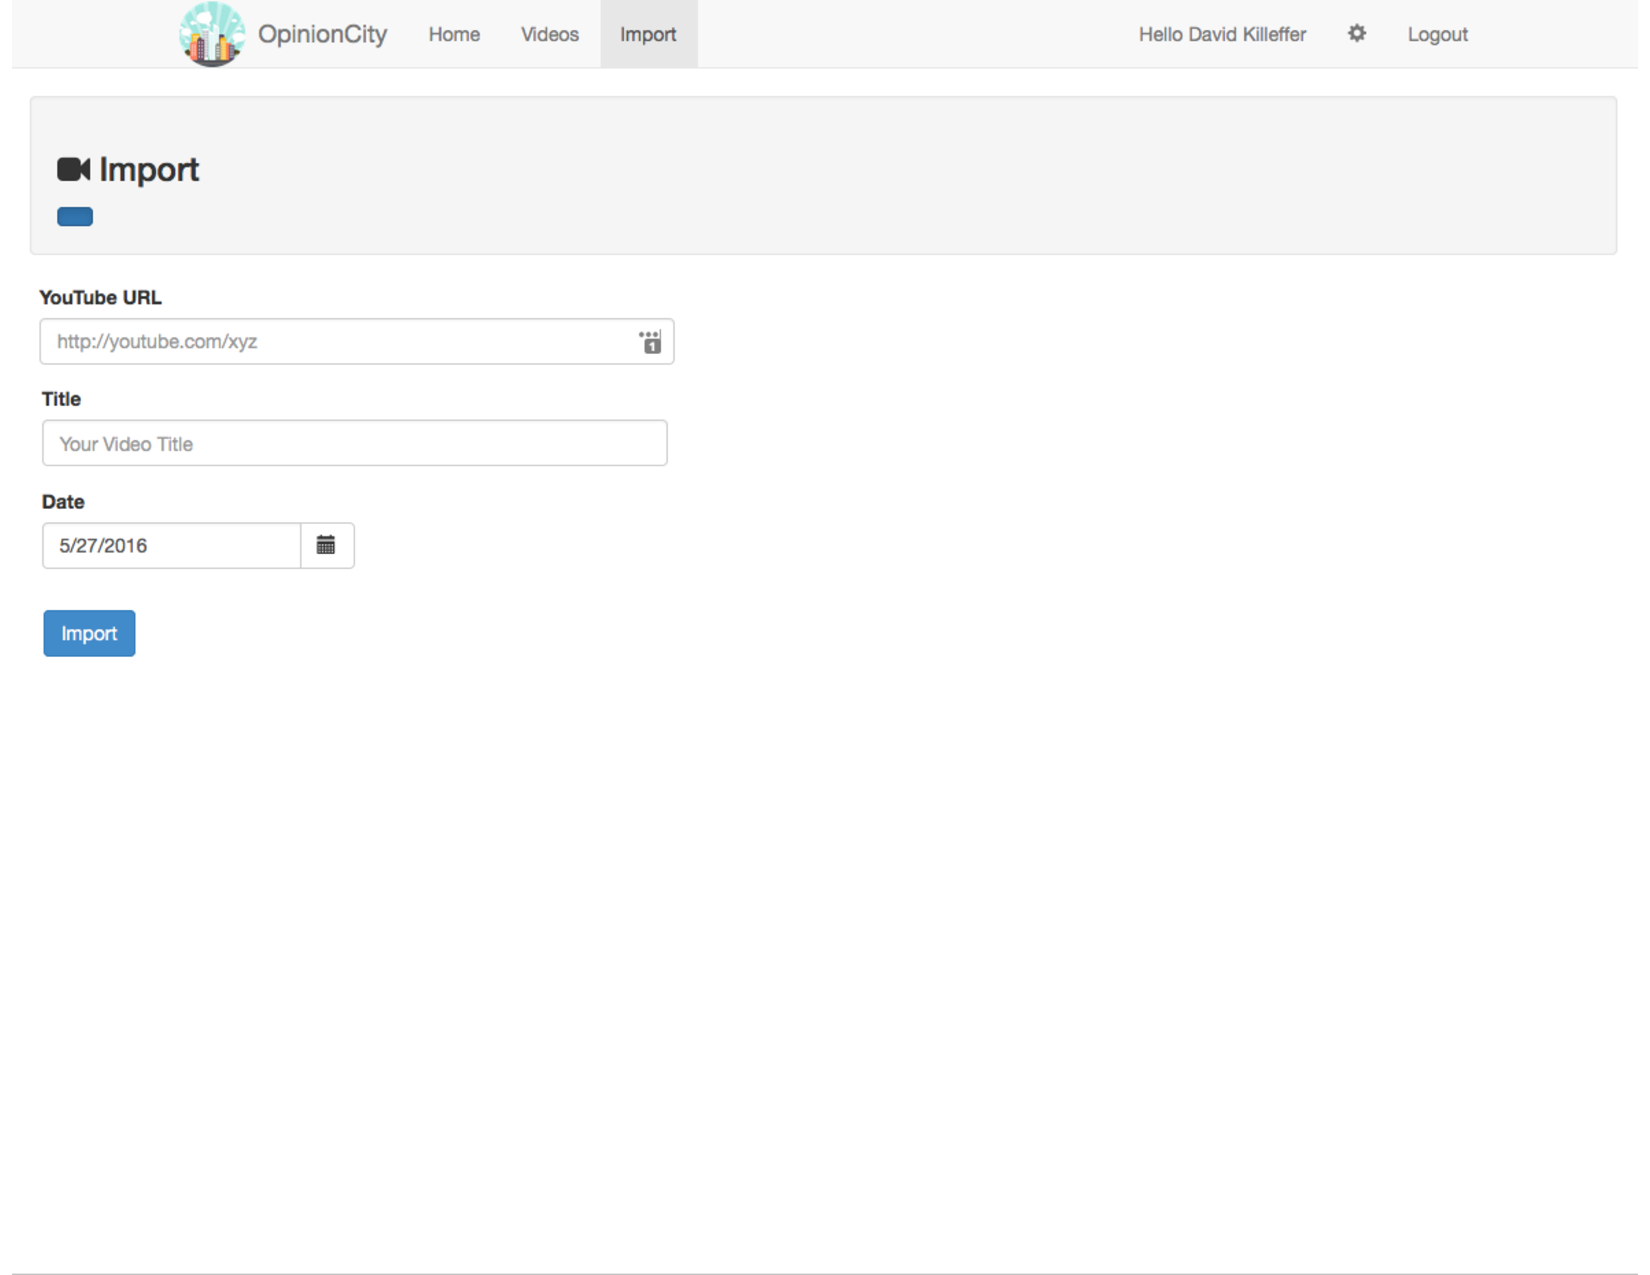
\includegraphics[width=\textwidth]{gfx/opinion-city/import1.pdf}
	\caption{\textit{(OpinionCity)} importing a video from \href{http://www.youtube.com}{YouTube} into OpinionCity} 
	\label{fig:opinioncity:importing-a-video-from-youtube}
\end{figure} 

\begin{figure}[ht]
	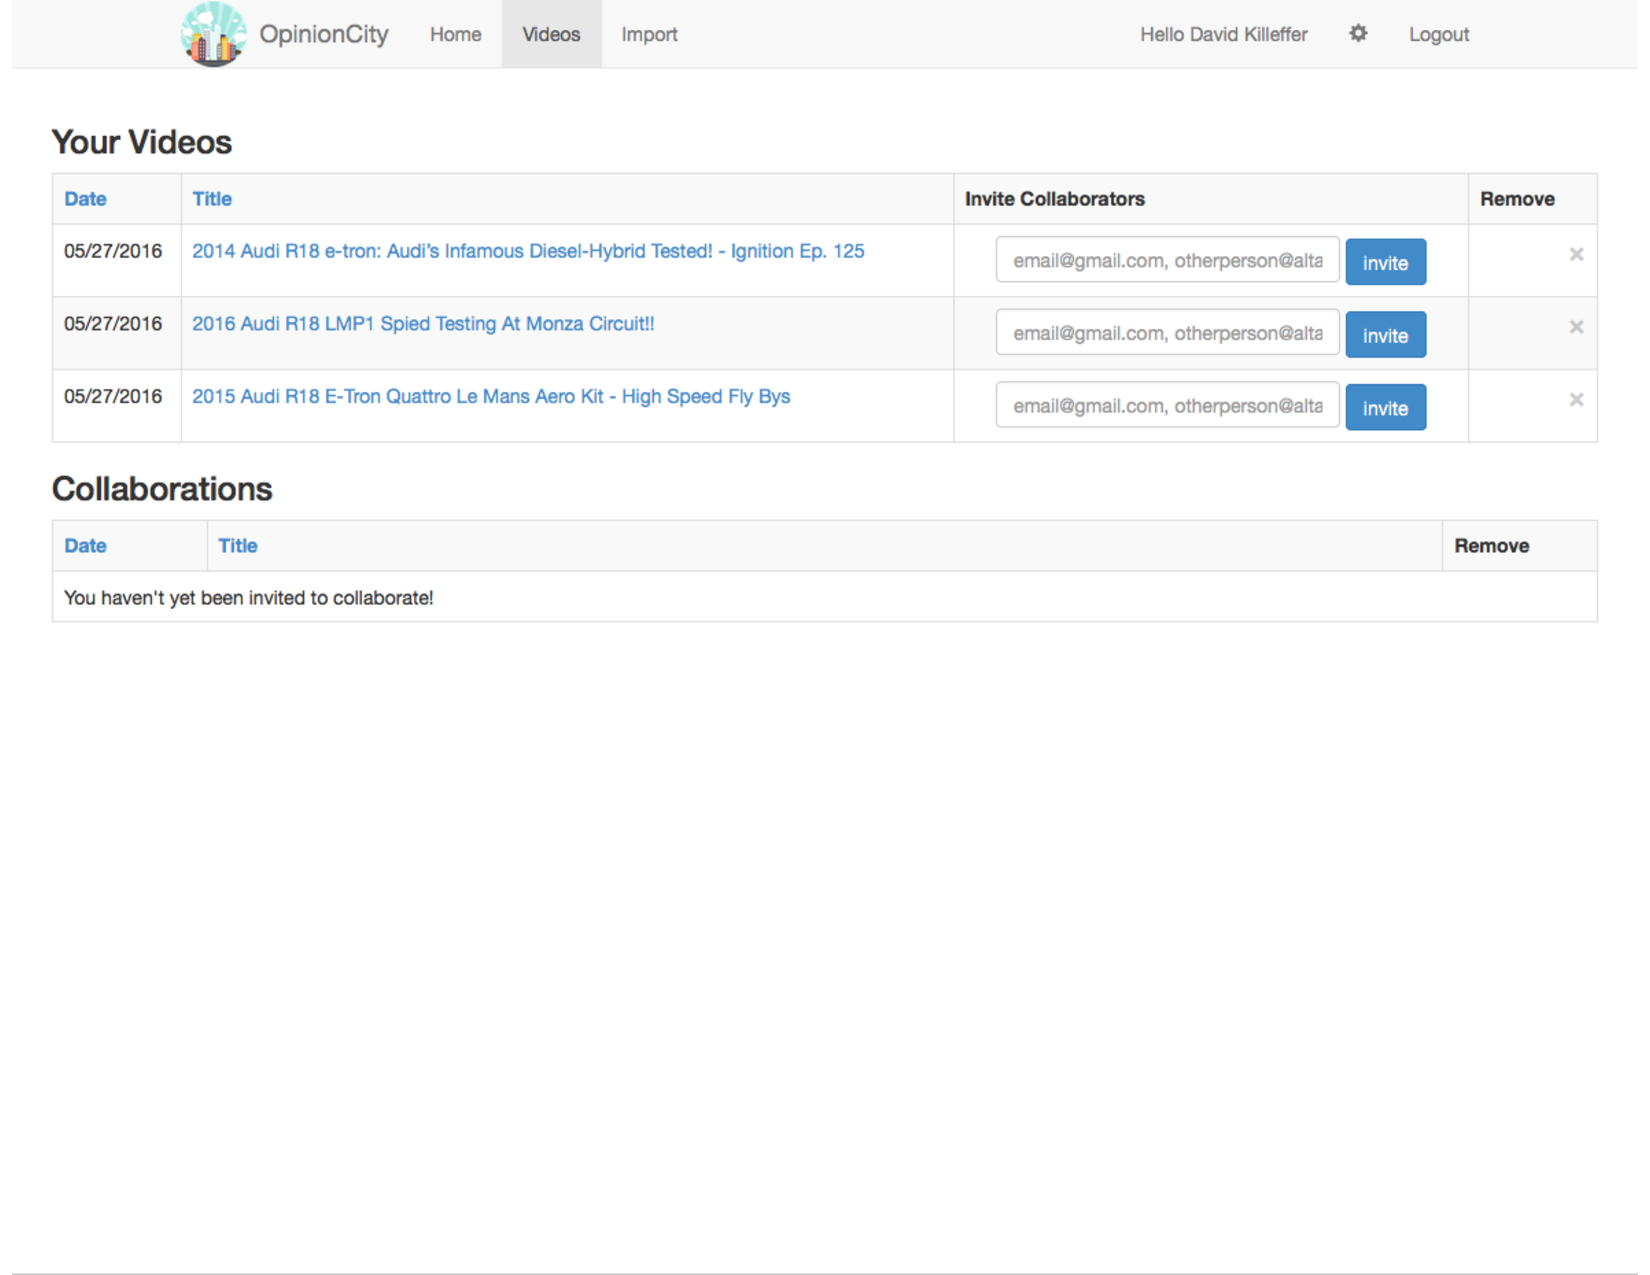
\includegraphics[width=\textwidth]{gfx/opinion-city/videolist1.pdf}
	\caption{\textit{(OpinionCity)} listing of all videos associated with a user account} 
	\label{fig:opinioncity:video-listing}
\end{figure}

\begin{figure}[ht]
	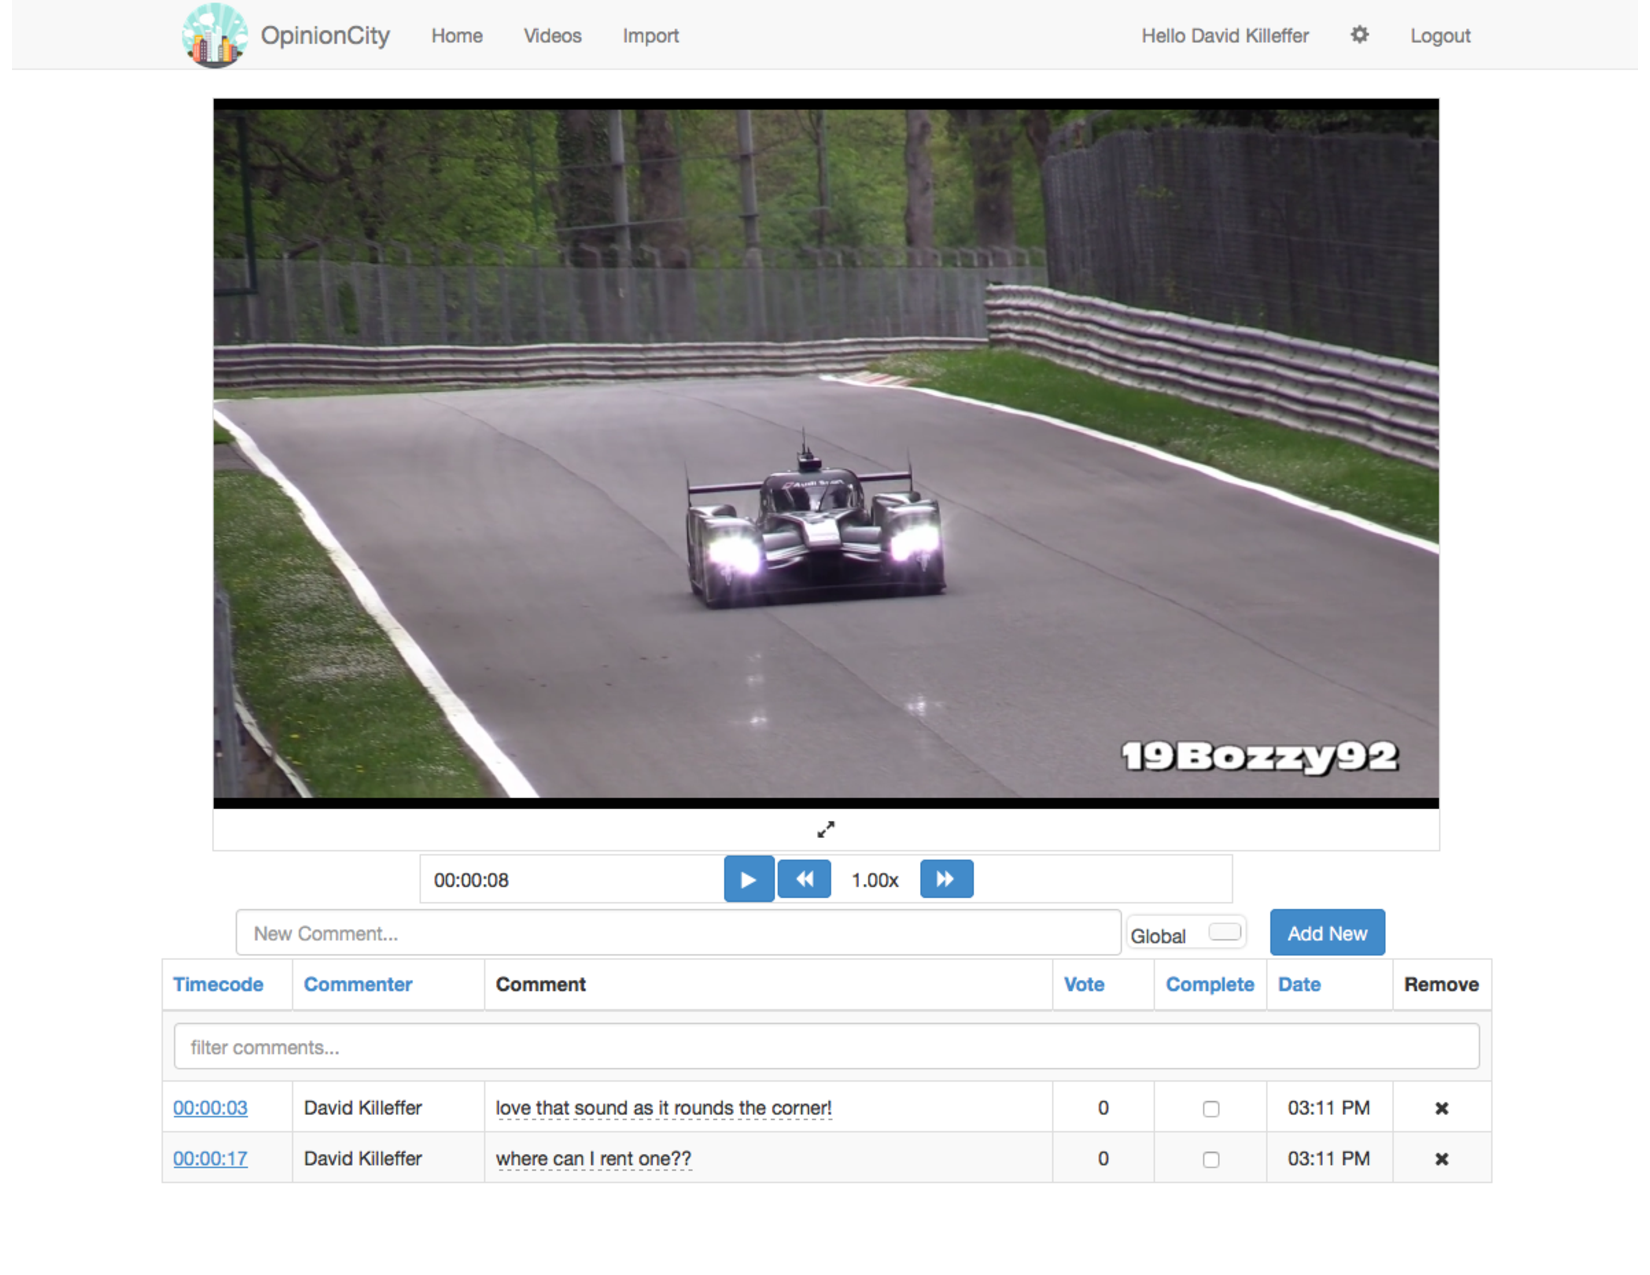
\includegraphics[width=\textwidth]{gfx/opinion-city/car2.pdf}
	\caption{\textit{(OpinionCity)} another view of adding video annotations} 
	\label{fig:opinioncity:adding-video-annotations-view2}
\end{figure}

%\href{http://opinion.city}{OpinionCity}, by Daniel P. Coffey: \href{mailto:danielpcoffey@gmail.com}{\nolinkurl{danielpcoffey@gmail.com} }, Spring 2015 \\
\textit{by Daniel P. Coffey: \href{mailto:danielpcoffey@gmail.com}{\nolinkurl{danielpcoffey@gmail.com} }, Spring 2015}

\href{http://opinion.city}{OpinionCity} is a website that was created by Daniel P. Coffey for a Digital Media Capstone project at Harvard Extension School.  It is a tool for real-time group feedback on videos that have been uploaded to YouTube and allows for collaborative, time-code based annotation of videos as well as whole-video annotations.  Users may select a video to "upload" to OpinionCity where the video from YouTube will play in an embedded player, and then users can add comments to the video at specific timecodes or apply their remarks to the entire video.  Users can also invite others to join in and comment on the video as well. 

While OpinionCity does allow for users to add annotations to specific parts of videos, it does not appear to allow for very granular annotations; specifically, a user may add an annotation at a specific part of the video denoting the "beginning" of an annotation, but cannot mark the "end" of the annotation.  This means that the annotation functionality is somewhat limited in that users are not able to define during what specific timeframe in a video a person is in, or where the video was shot, etc.  For annotating relatively shorter-length videos such as are often found on YouTube, this may be fine, but for annotating entire tape-length (typically 60-120 minutes or occasionally longer), this mechanism would be insufficient. 

Additionally, OpinionCity does not appear to have any search functionality.  Users may add annotations to videos, but there is no mechanism whereby they can then later search what annotations have been added.  The project seems to have focused much more on the real-time aspects of commenting on a video, where a group of interested people may be watching a video at the same time and then making annotations and comments, and quickly viewing what others have likewise annotated and commented.  Here are some screenshots of OpinionCity:

%\\ 
%{\centering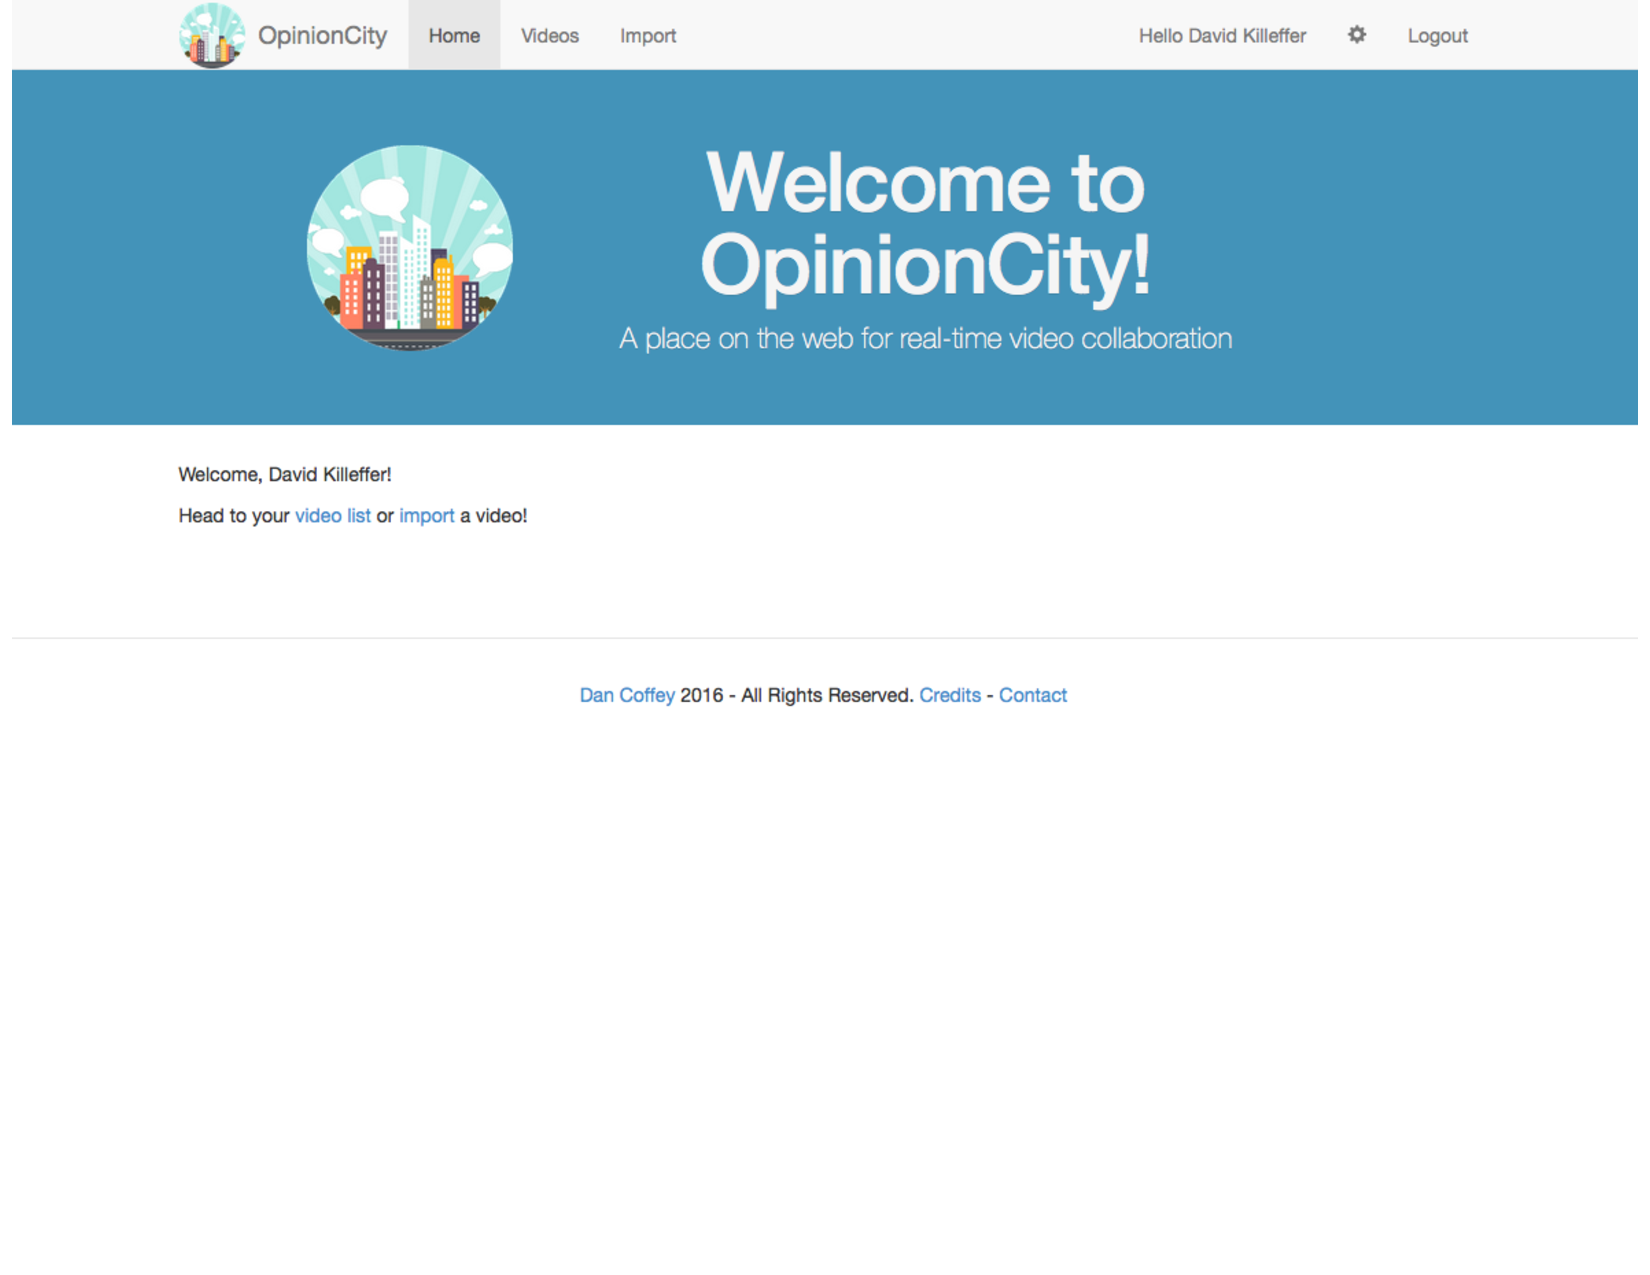
\includegraphics[width=1\textwidth]{gfx/opinion-city/homepage1.pdf}} \\
%{\centering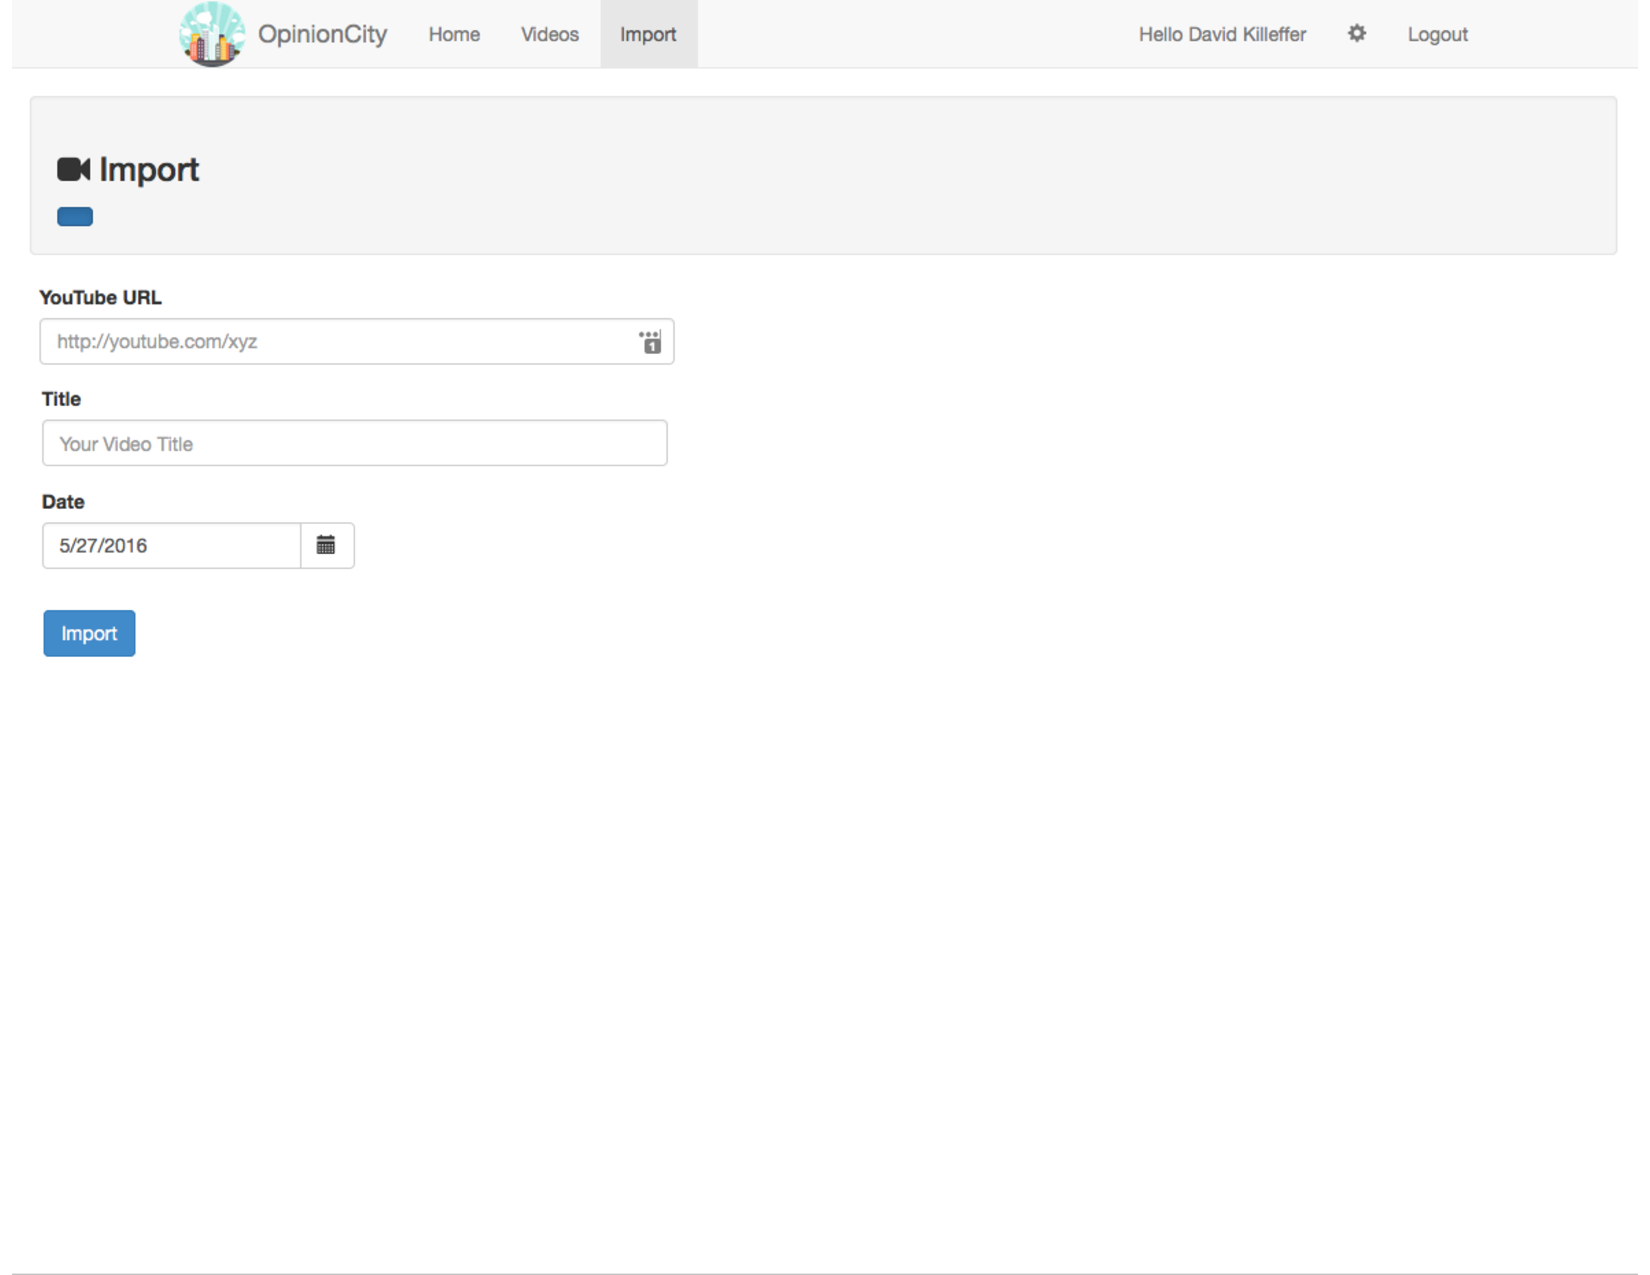
\includegraphics[width=1\textwidth]{gfx/opinion-city/import1.pdf}} \\
%{\centering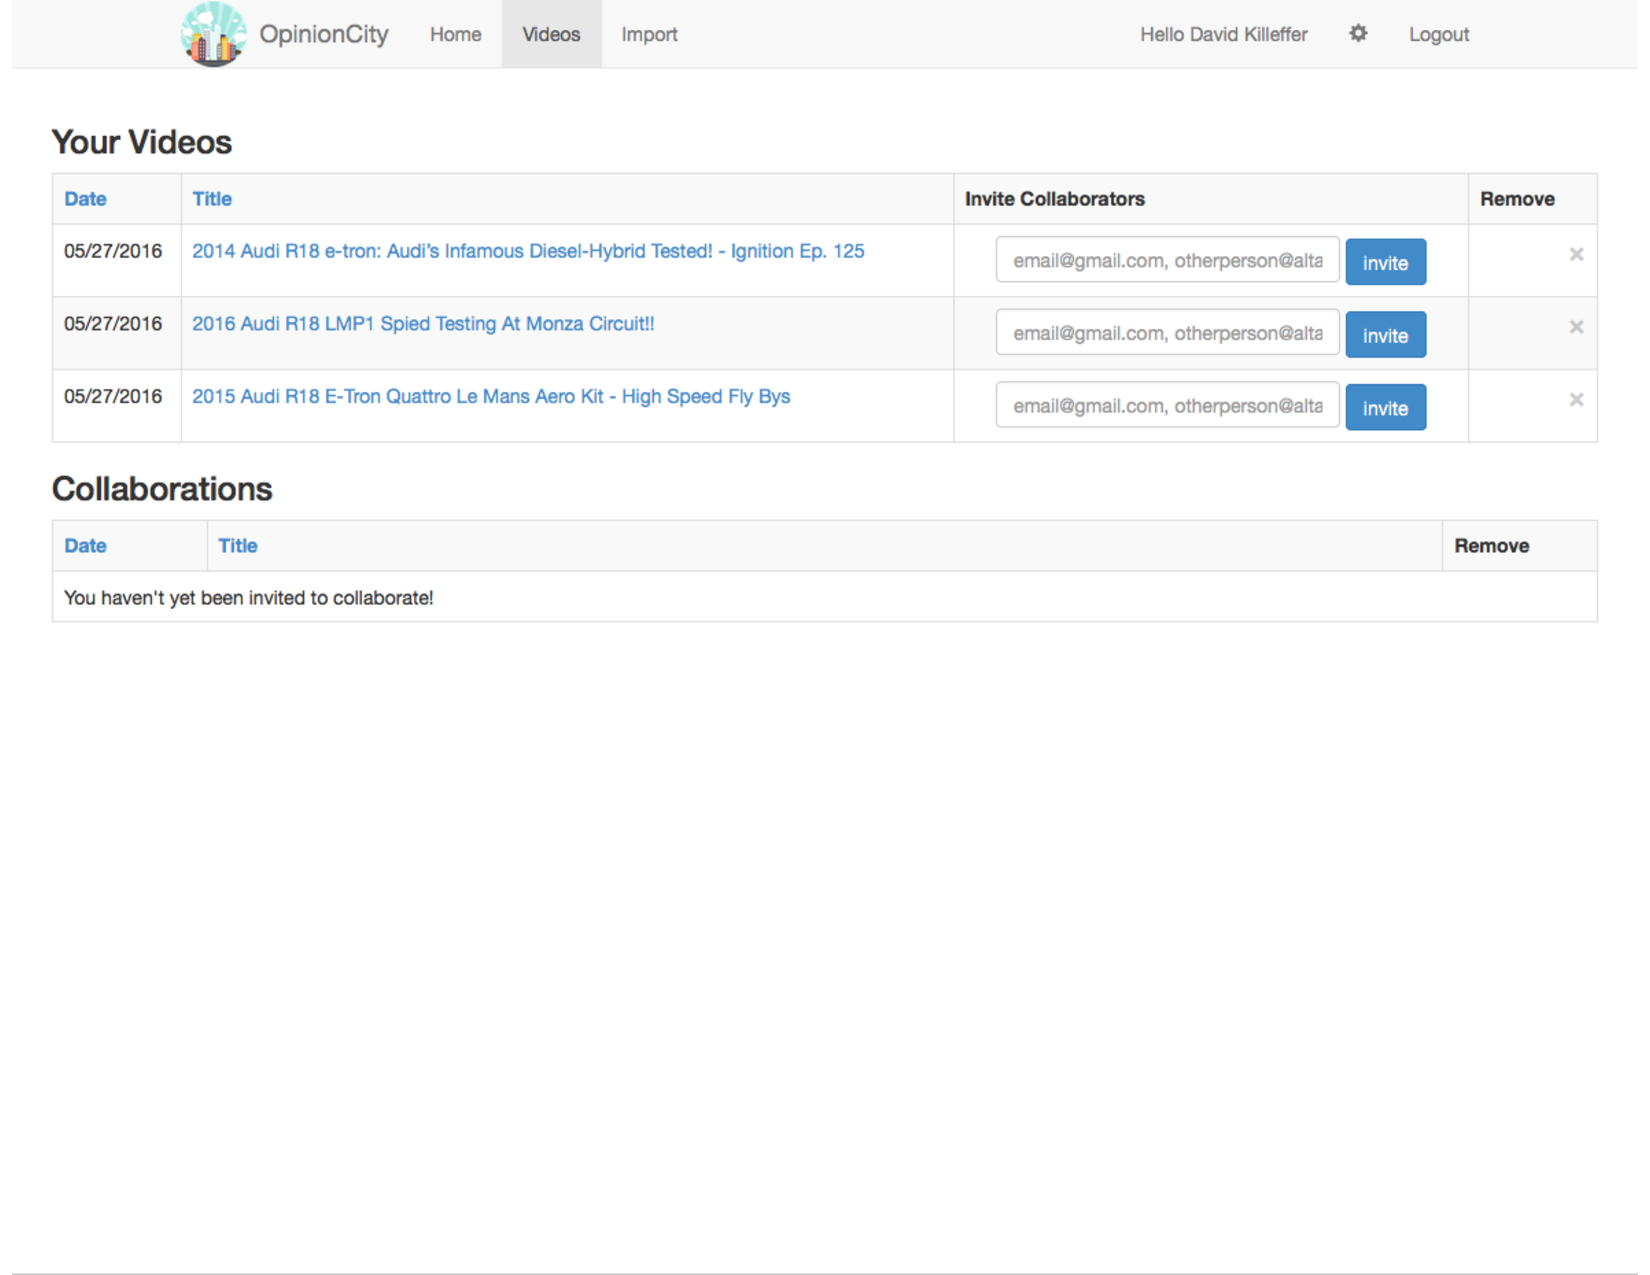
\includegraphics[width=1\textwidth]{gfx/opinion-city/videolist1.pdf}} \\
%{\centering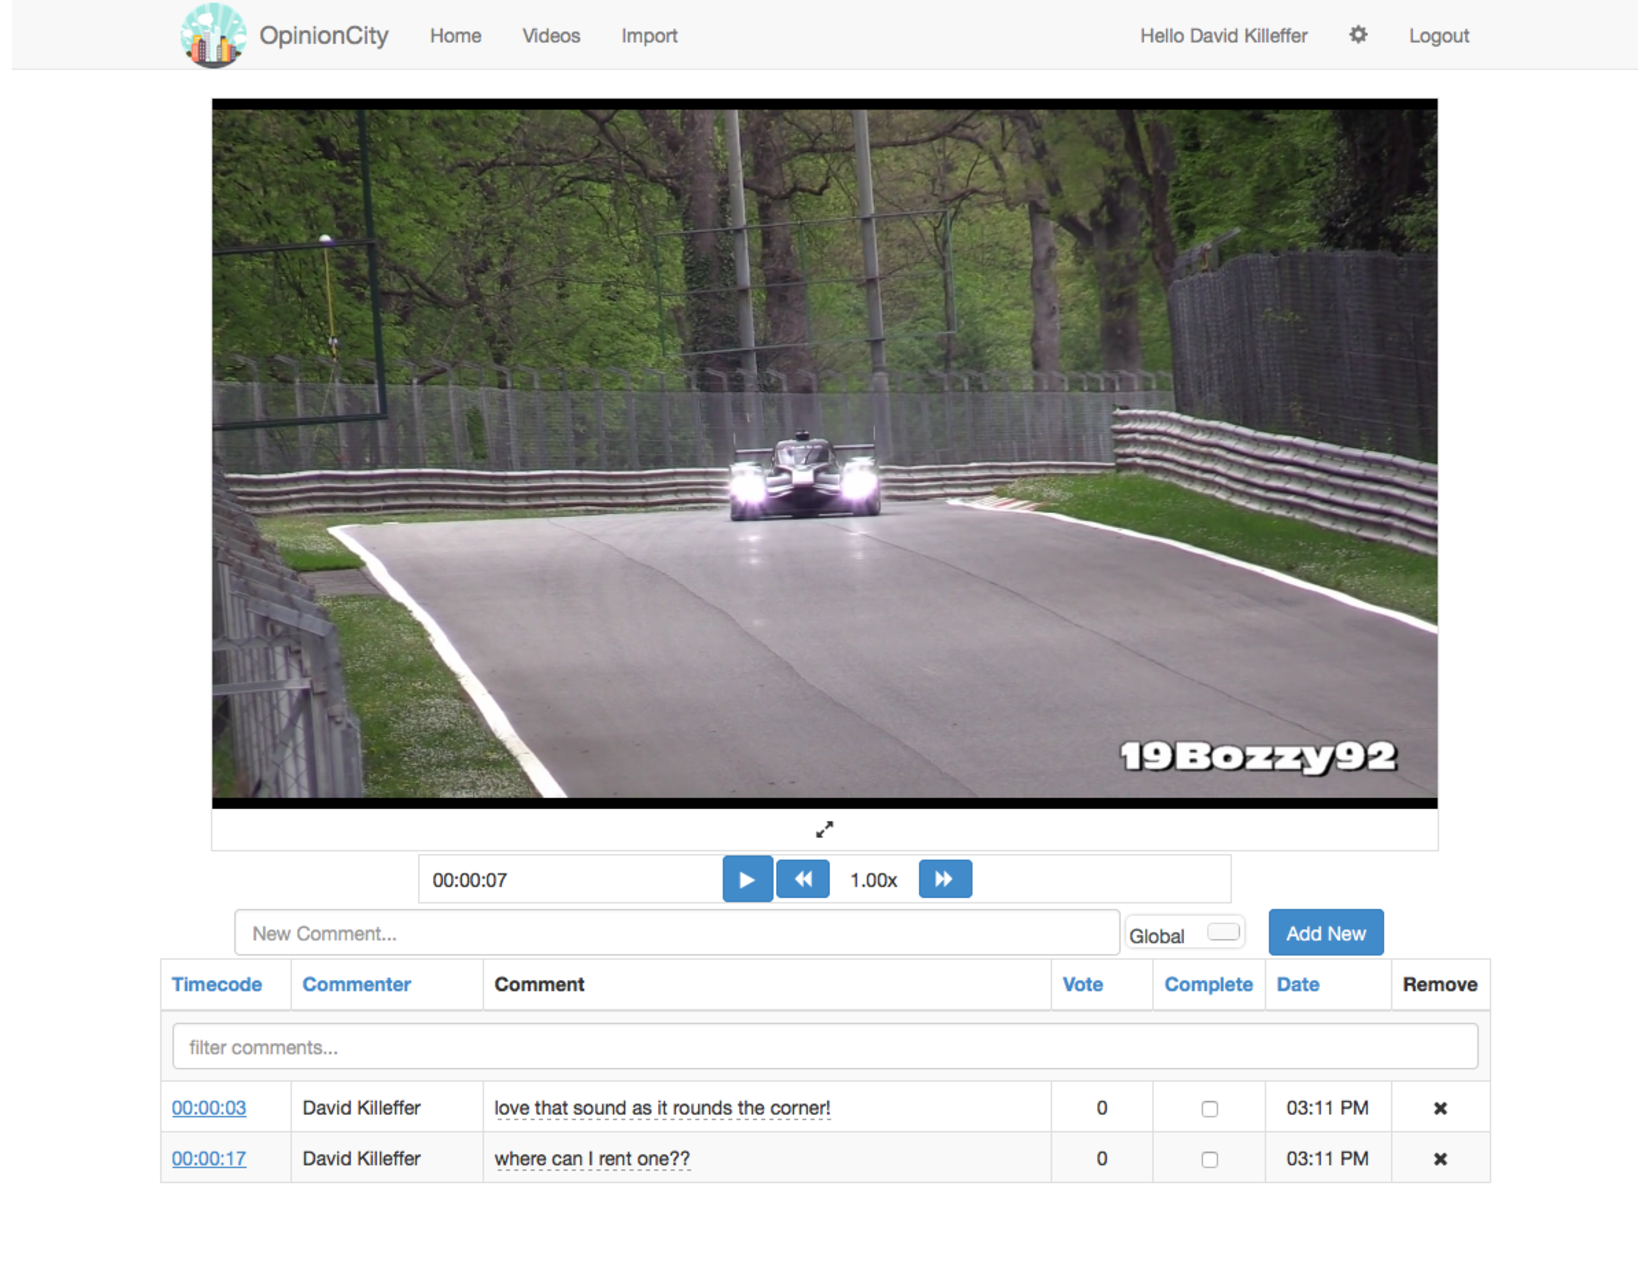
\includegraphics[width=1\textwidth]{gfx/opinion-city/car1.pdf}} \\
%{\centering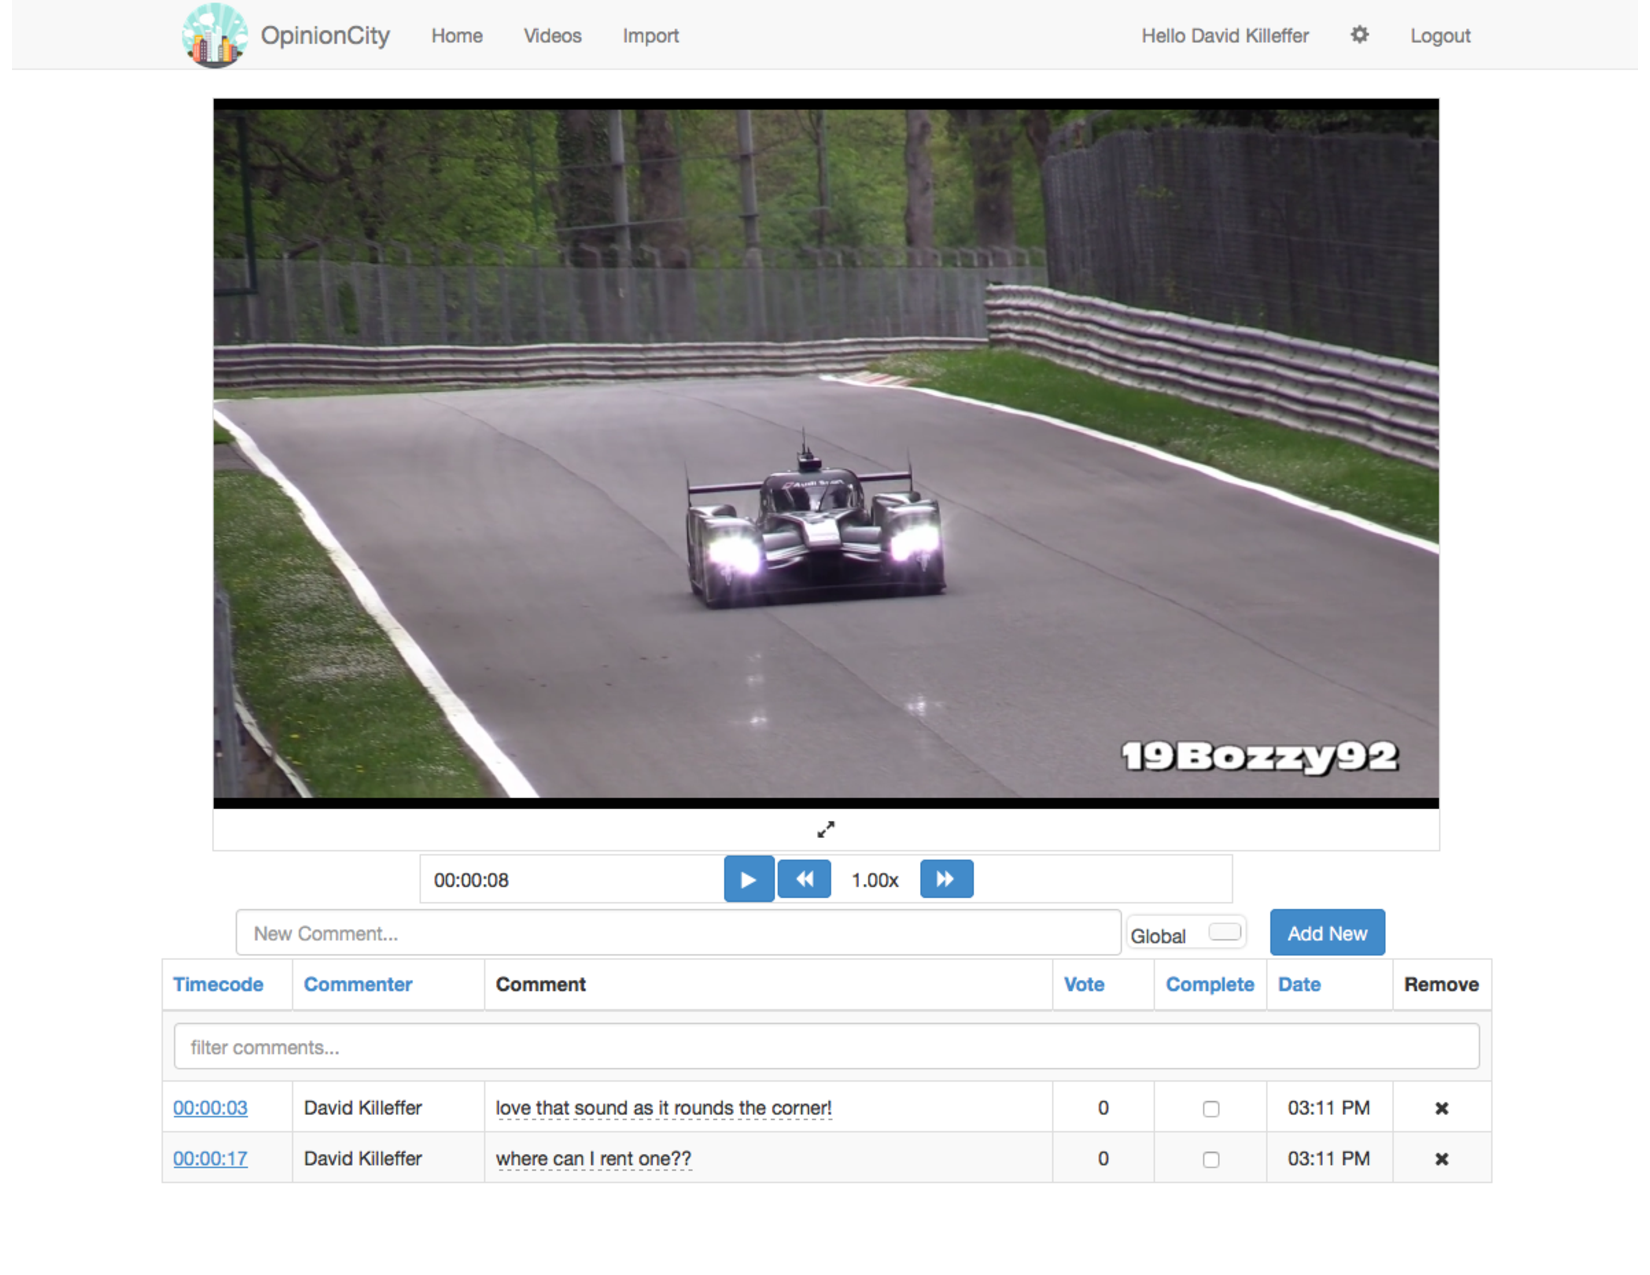
\includegraphics[width=1\textwidth]{gfx/opinion-city/car2.pdf}} \\

%{\centering
%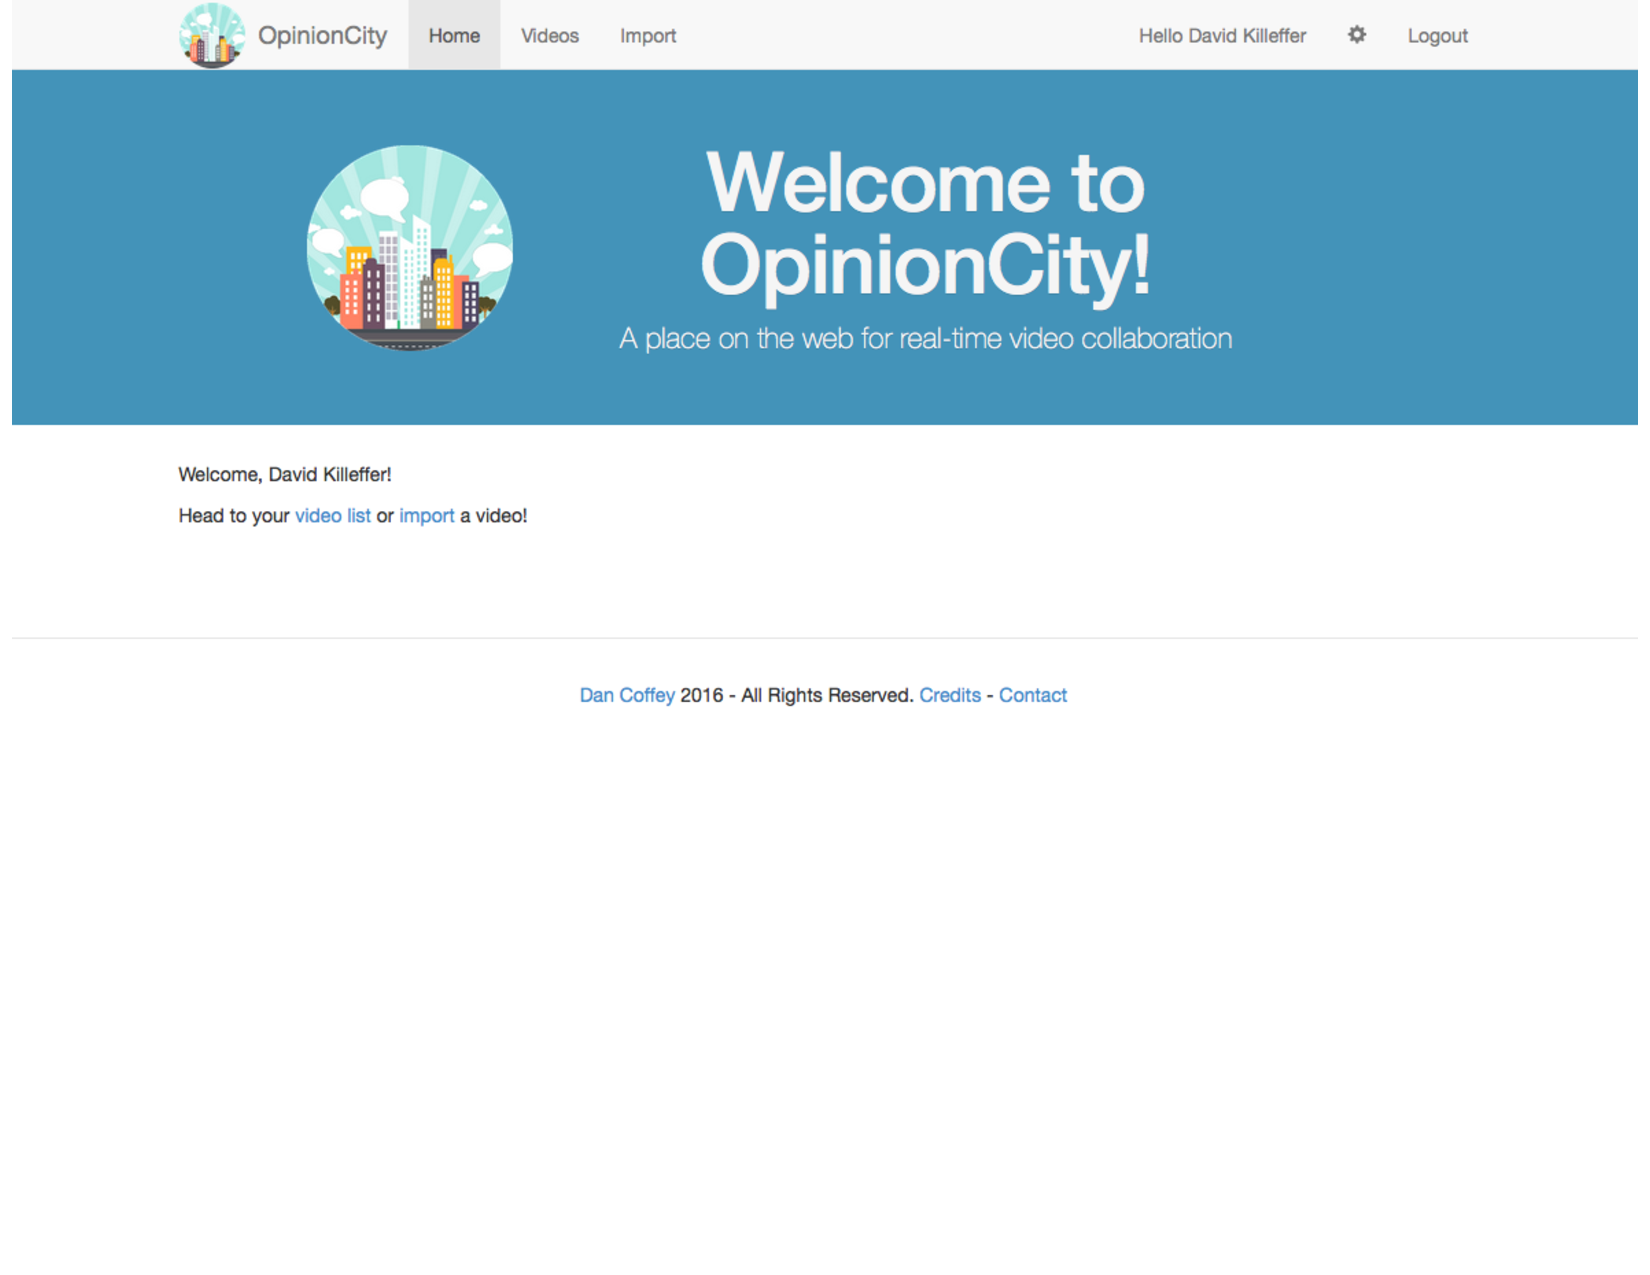
\includegraphics[width=1\textwidth]{gfx/opinion-city/homepage1.pdf} \\
%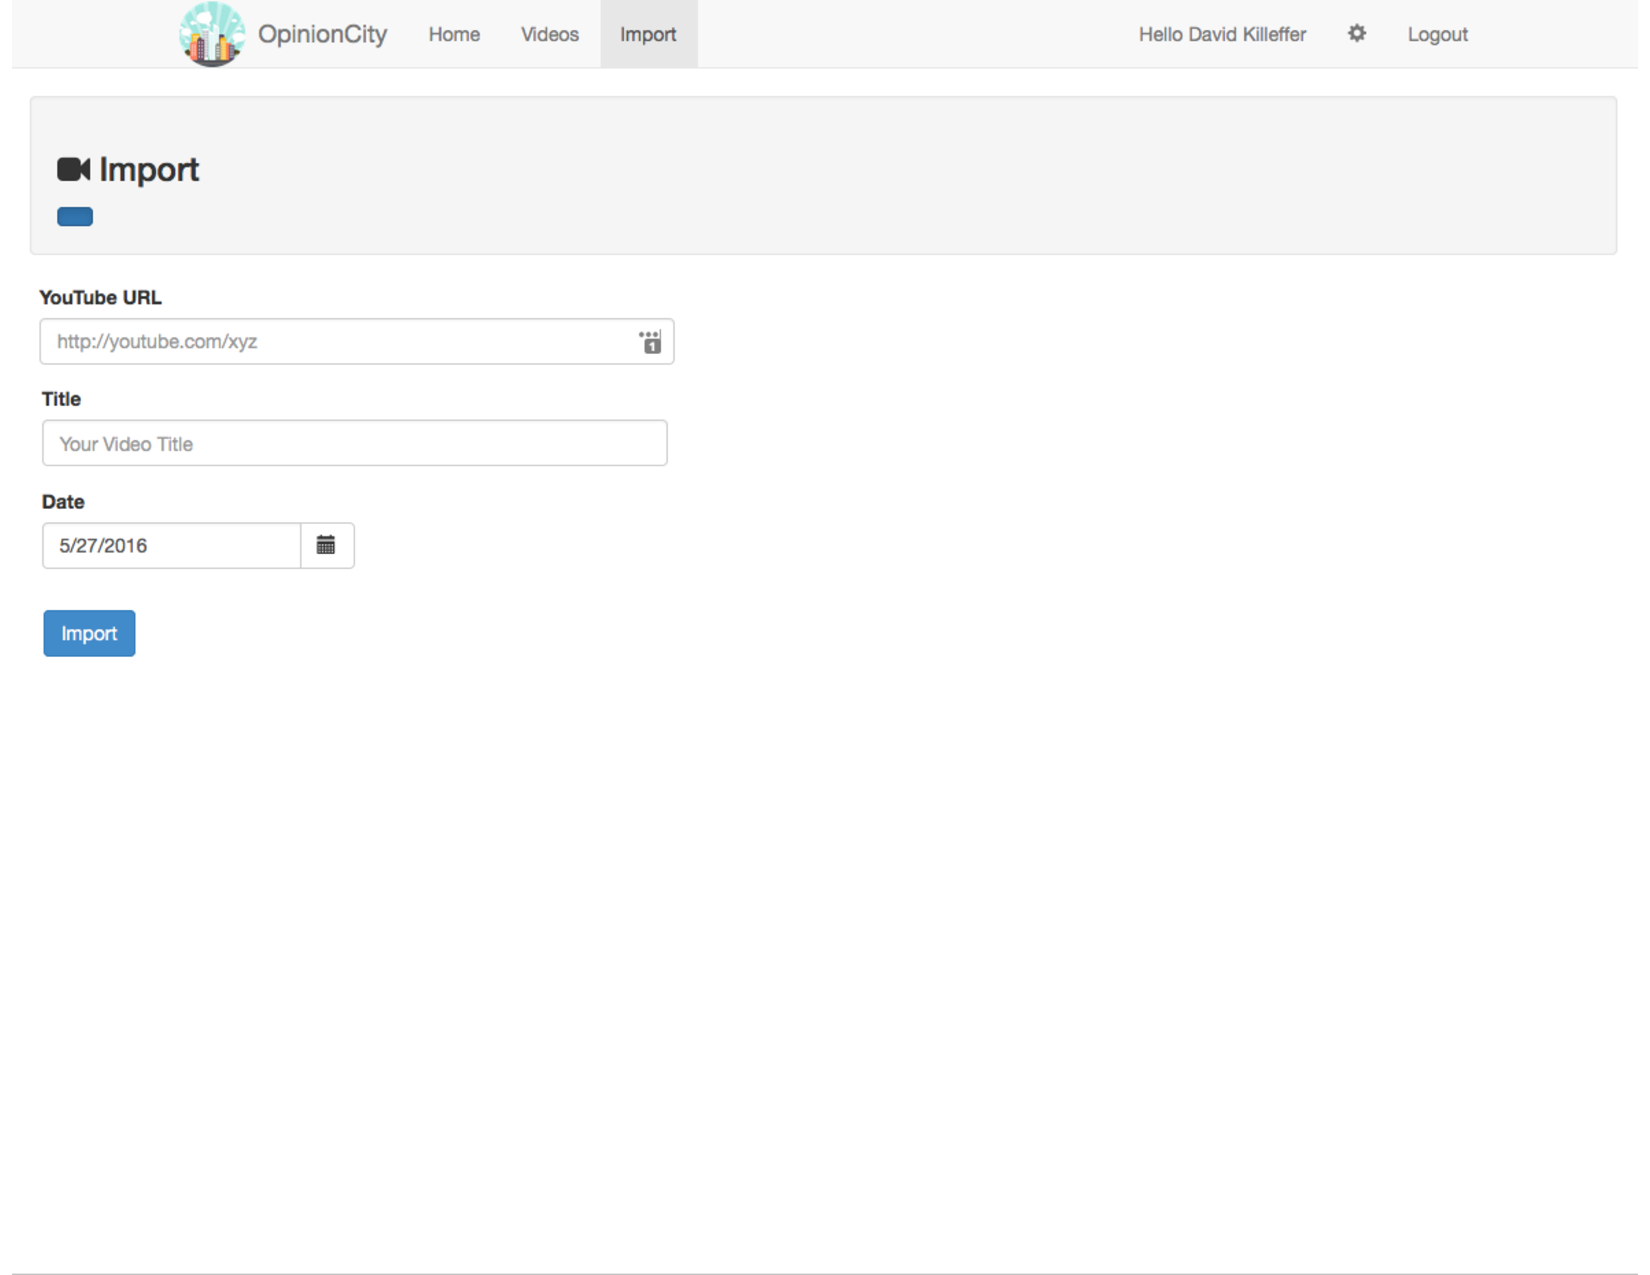
\includegraphics[width=1\textwidth]{gfx/opinion-city/import1.pdf} \\
%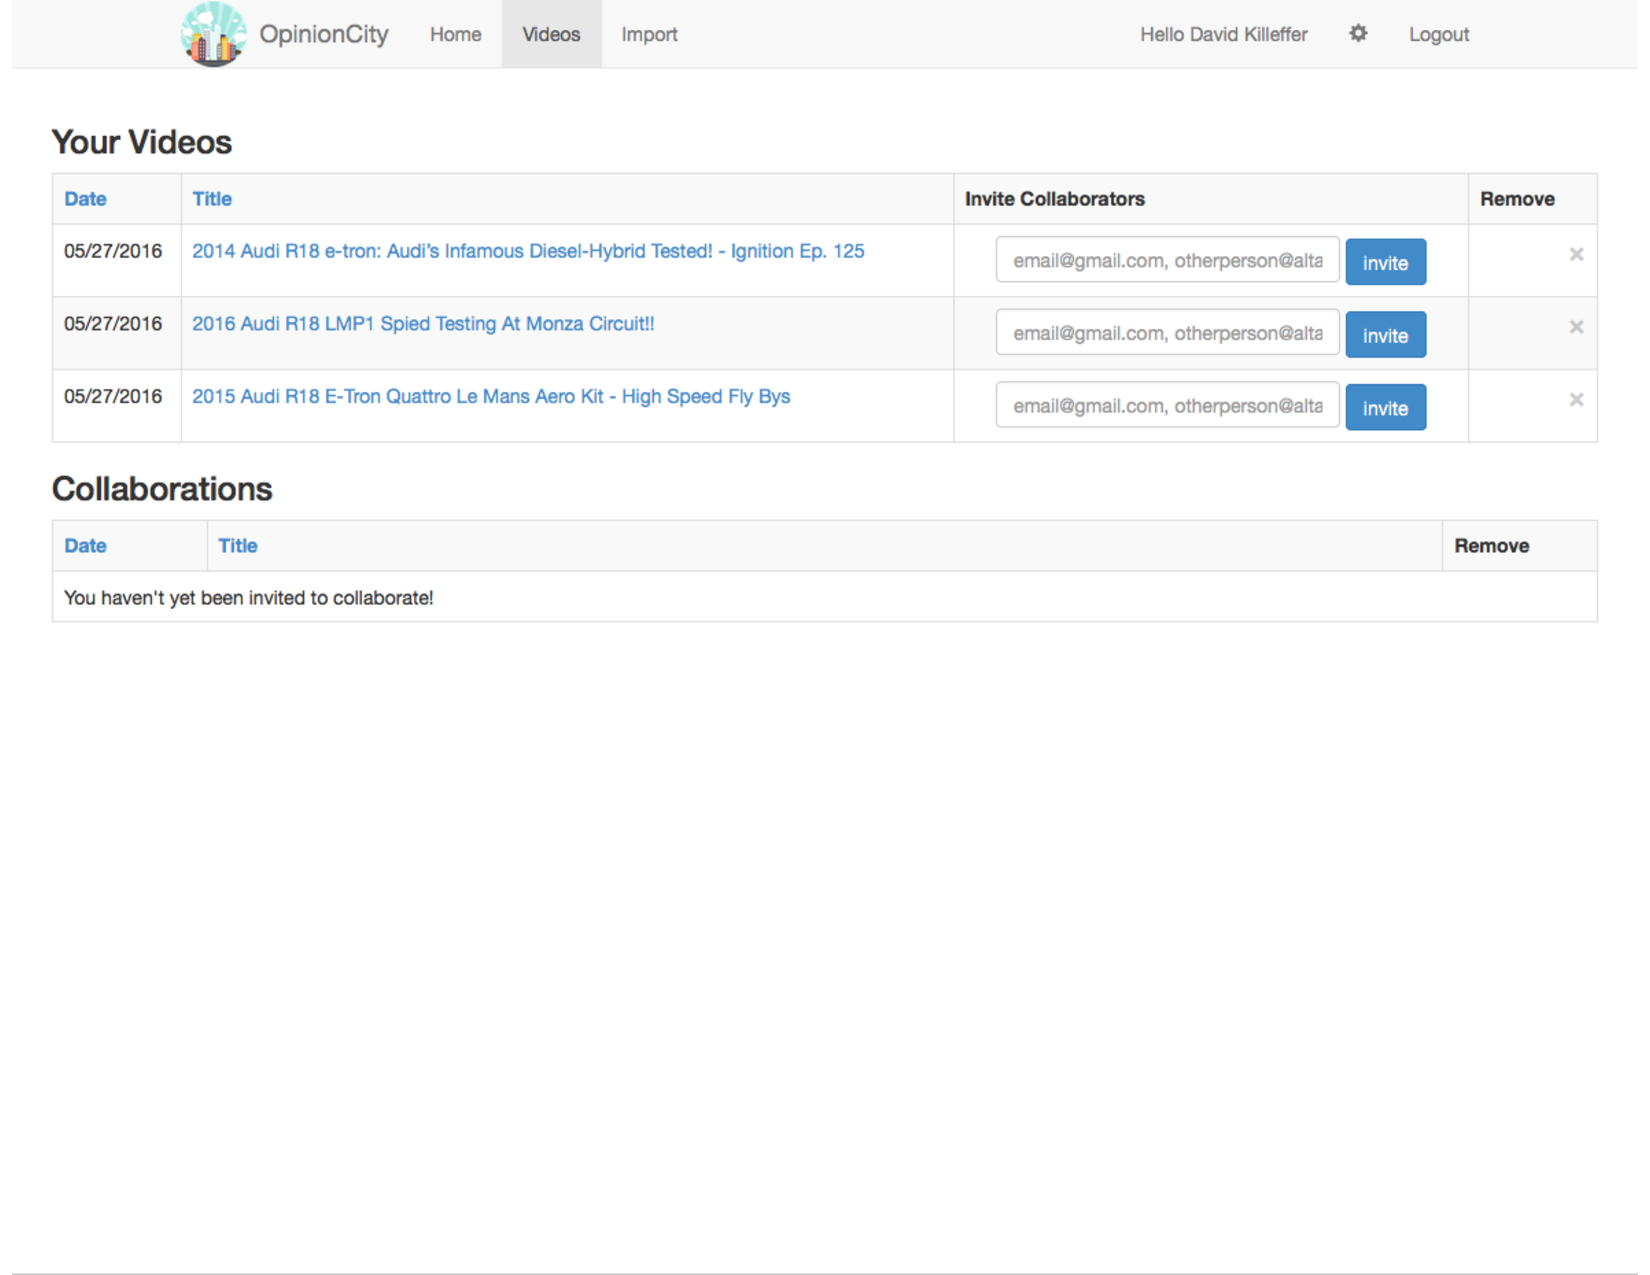
\includegraphics[width=1\textwidth]{gfx/opinion-city/videolist1.pdf} \\
%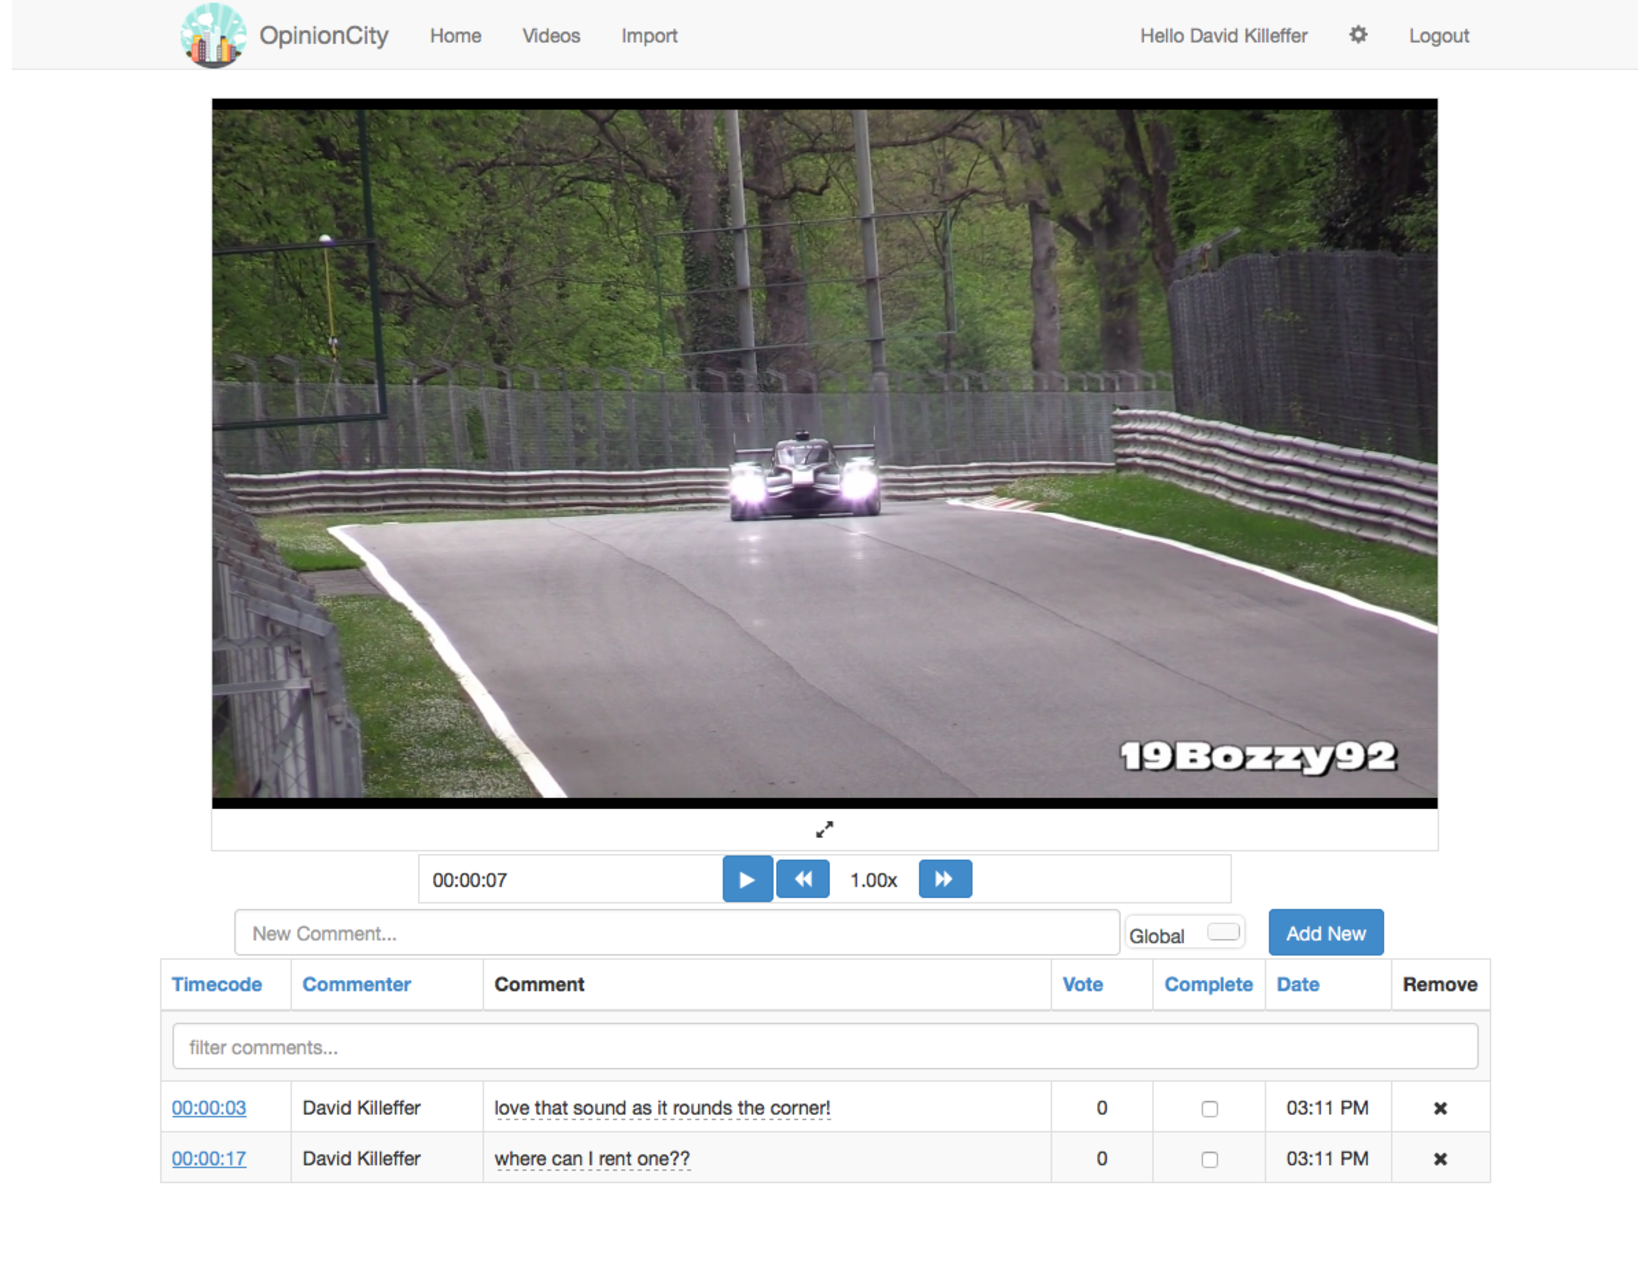
\includegraphics[width=1\textwidth]{gfx/opinion-city/car1.pdf} \\
%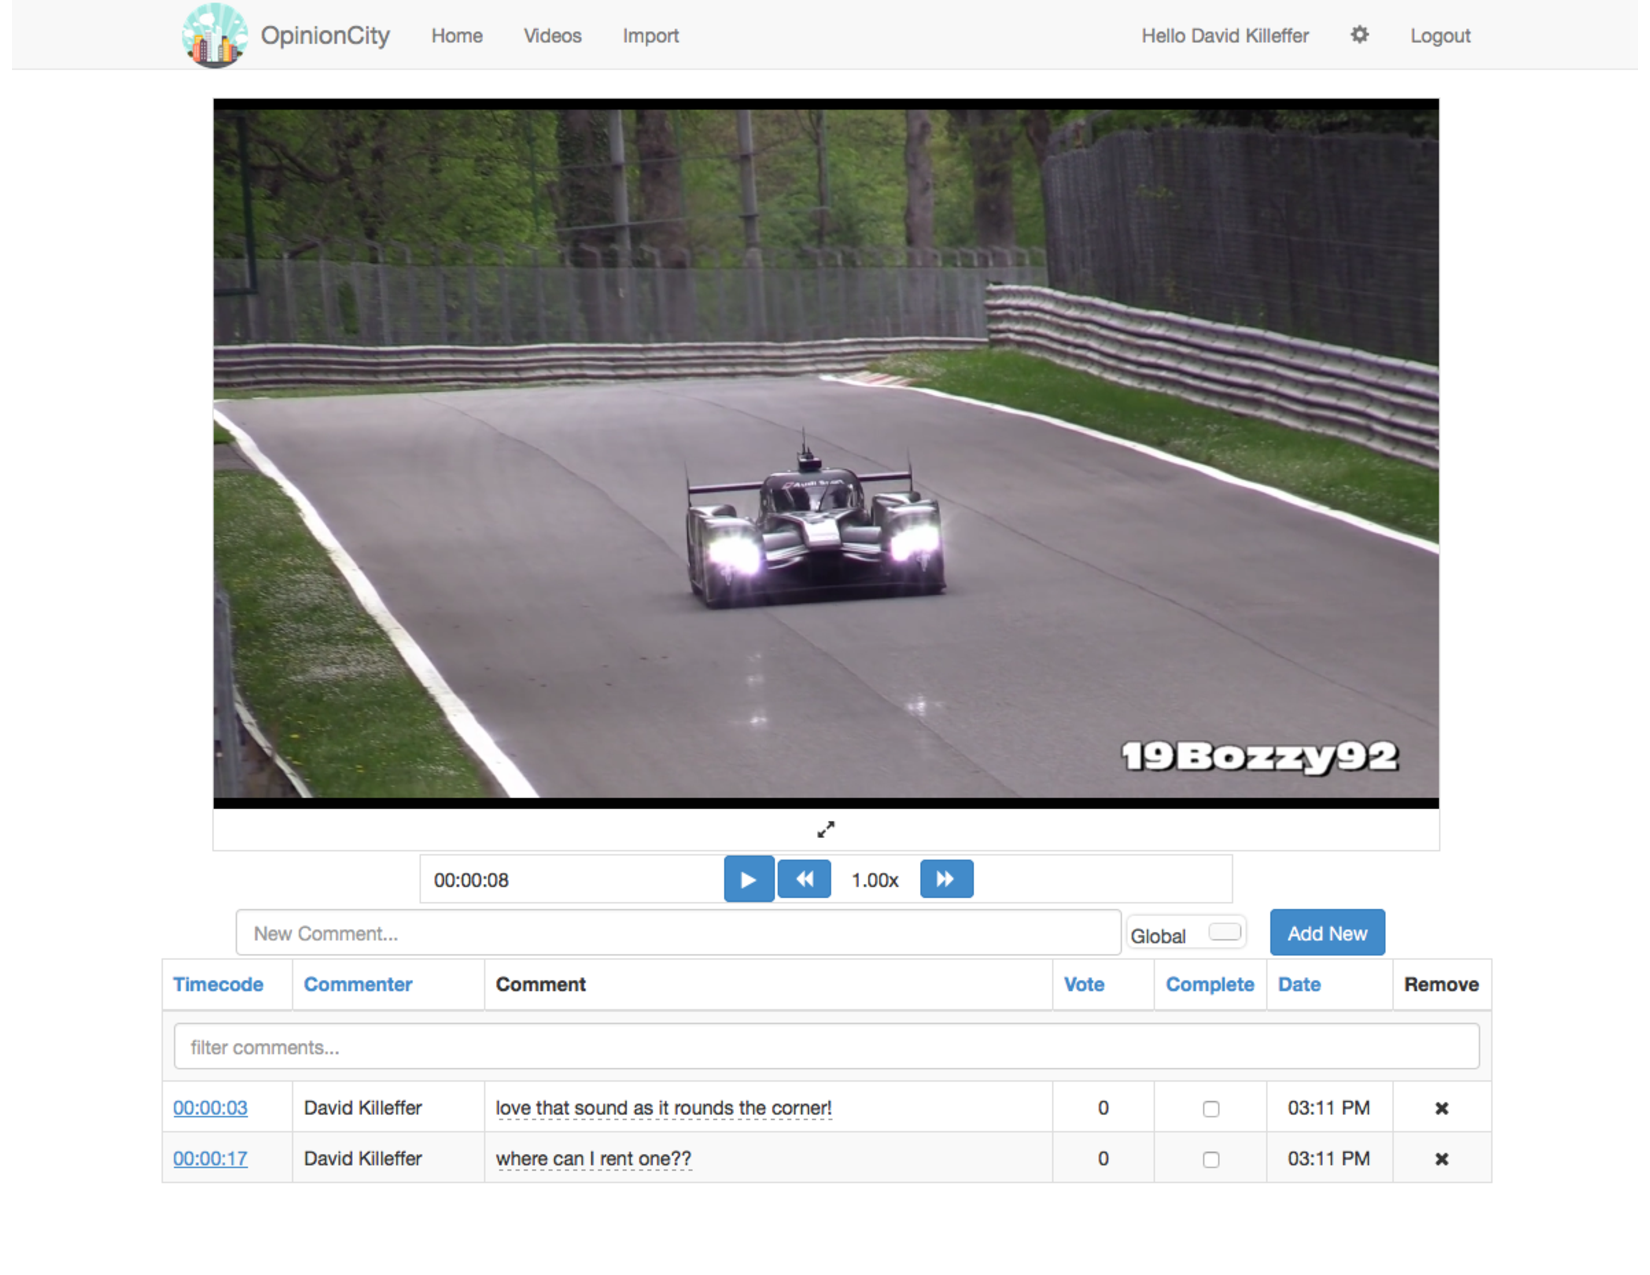
\includegraphics[width=1\textwidth]{gfx/opinion-city/car2.pdf} \\
%}



\begin{figure}[!ht]
	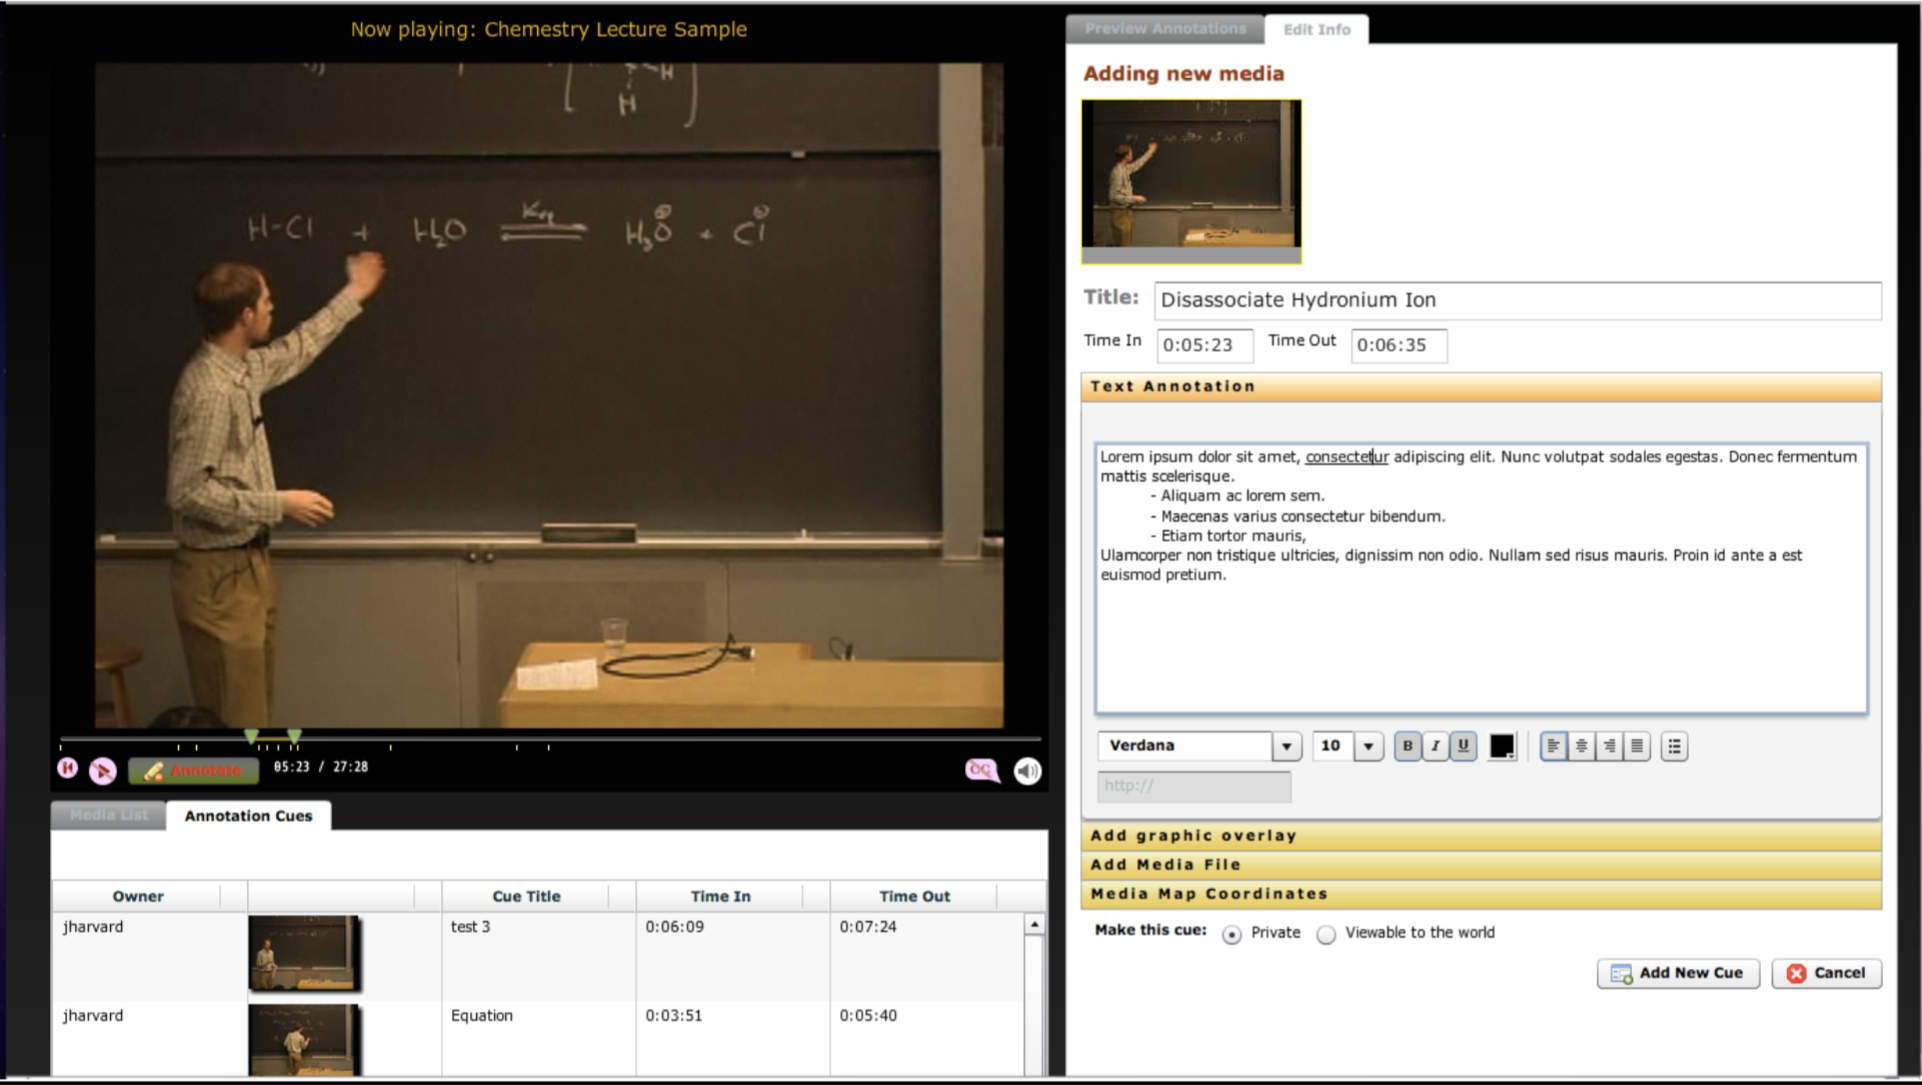
\includegraphics[width=\textwidth]{gfx/mvat/mvat-annotation-edit-view.png}
	\caption{\textit{(MVAT)} video annotation edit view} 
	\label{fig:mvat:video-annotation-edit-view}
\end{figure} 

\begin{figure}[!ht]
	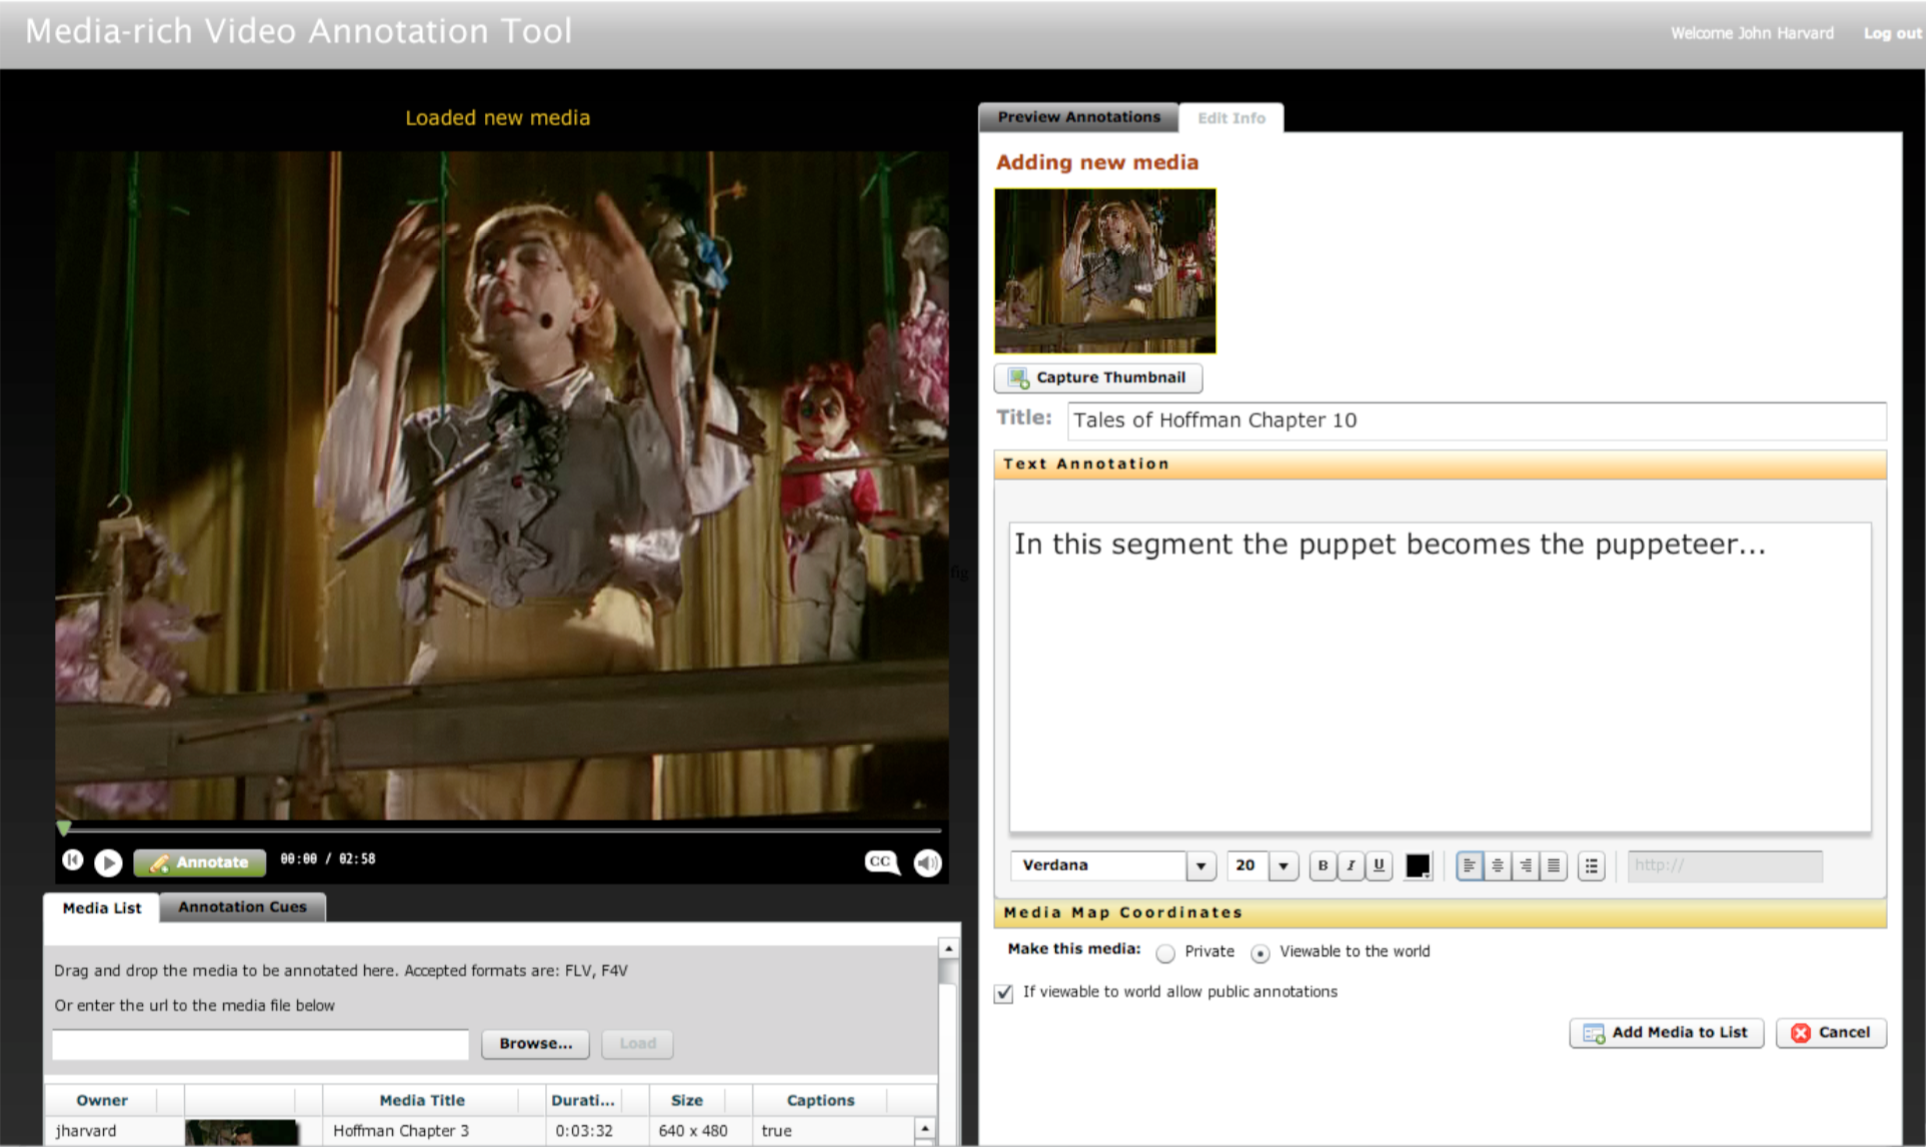
\includegraphics[width=\textwidth]{gfx/mvat/mvat-loading-video-adding-metadata.png}
	\caption{\textit{(MVAT)} adding video metadata view} 
	\label{fig:mvat:adding-video-metadata}
\end{figure} 

\begin{figure}[!ht]
	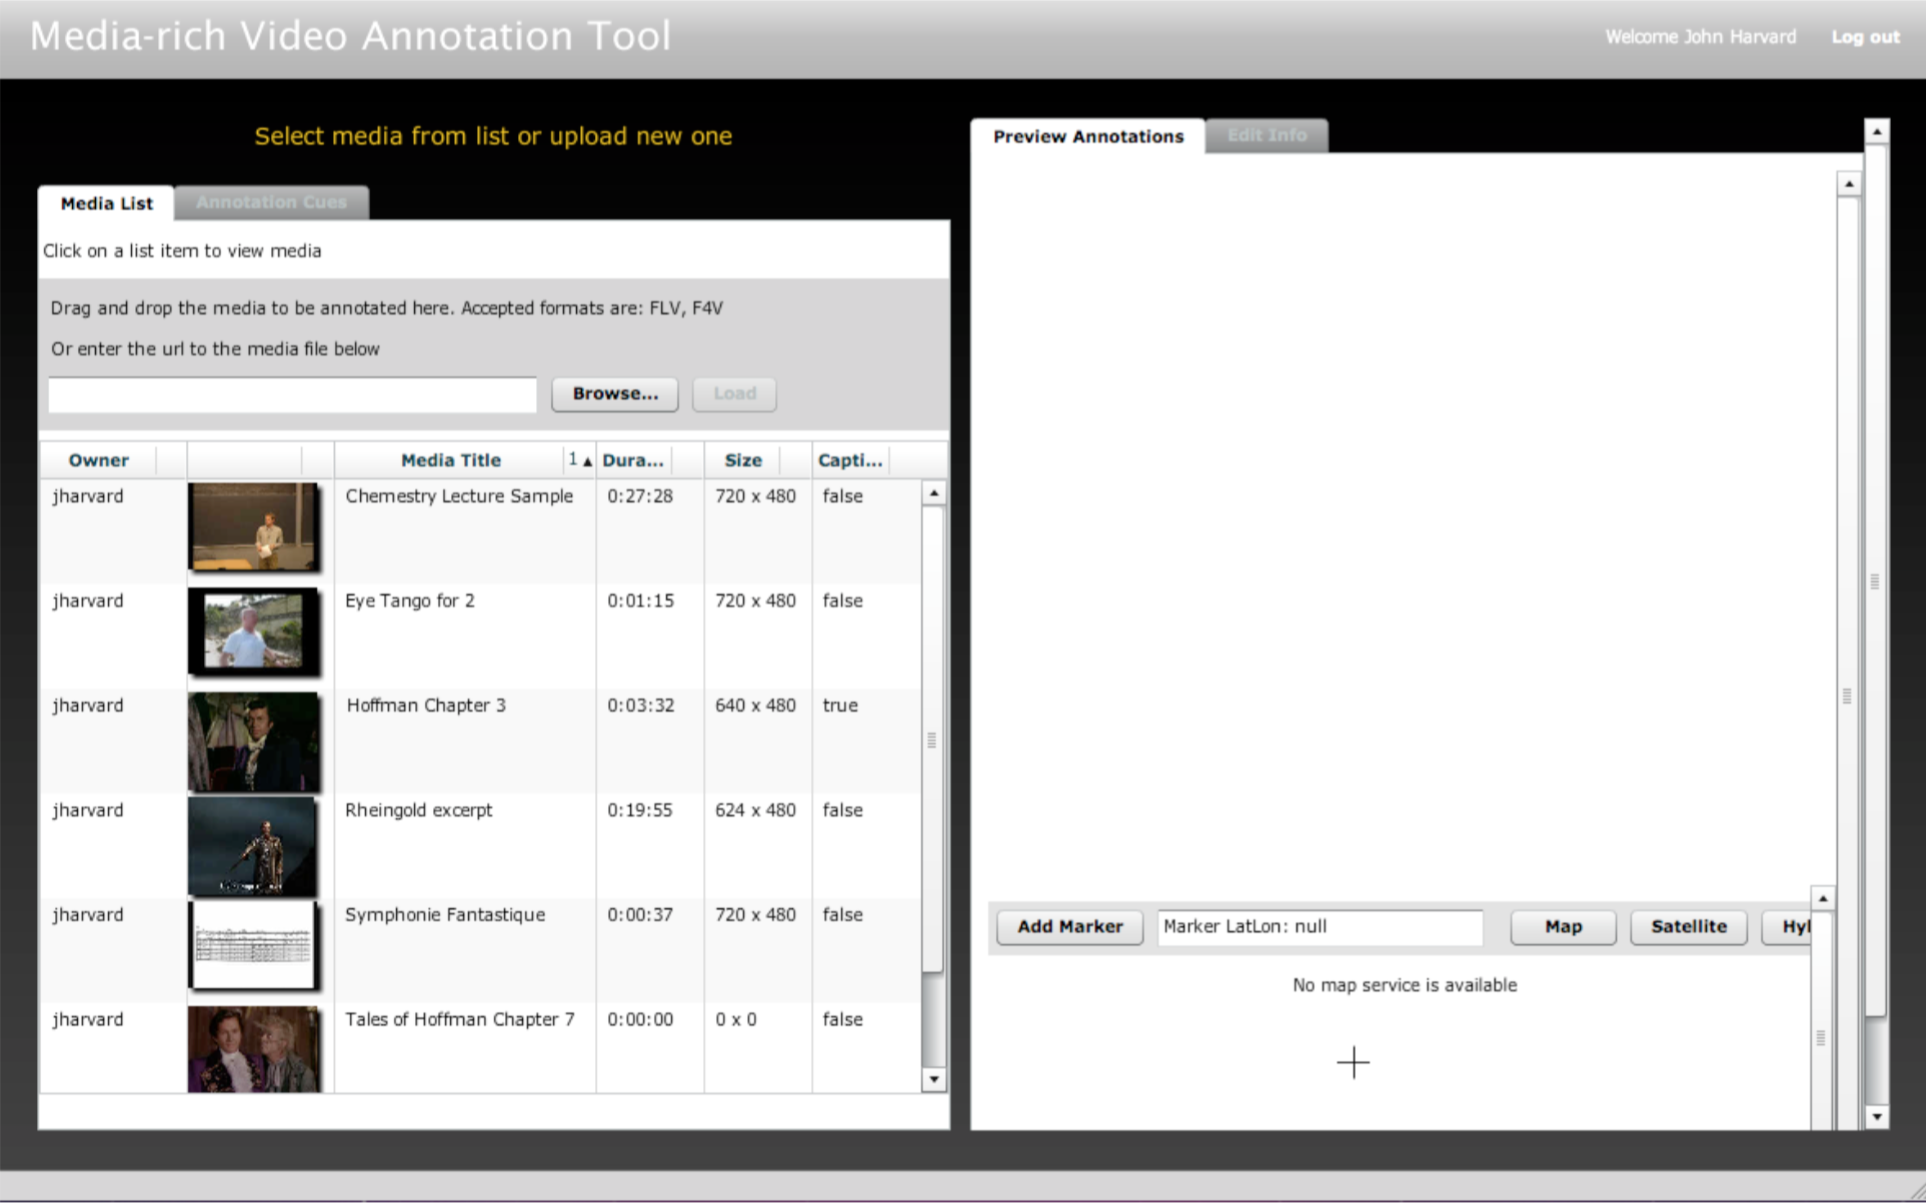
\includegraphics[width=\textwidth]{gfx/mvat/mvat-video-management}
	\caption{\textit{(MVAT)} video management view} 
	\label{fig:mvat:video-management-view}
\end{figure}

\section{Media-rich Video Annotation Tool (MVAT)}
\label{sec:priorwork:media-rich-video-annotation-tool}

%\item \textit{Media-rich Video Annotation Tool (MVAT)}, by Philip Desenne: \href{mailto:desenne@fas.harvard.edu}{\nolinkurl{desenne@fas.harvard.edu} }, May 2012 \\
%\textit{Media-rich Video Annotation Tool (MVAT)}, by Philip Desenne: \href{mailto:desenne@fas.harvard.edu}{\nolinkurl{desenne@fas.harvard.edu} }, May 2012
\textit{by Philip Desenne: \href{mailto:desenne@fas.harvard.edu}{\nolinkurl{desenne@fas.harvard.edu} }, May 2012}

The Media-rich Video Annotation Tool (MVAT) is a prototype tool developed by Philip Desenne as part of an A.L.M. in Information Technology thesis project at Harvard Extension School.  Motivation for the development of the MVAT stemmed from Desenne's work as an Academic Technologies Product Manager to support learning and simplify the process of creating and sharing video annotations amongst students in a pedagogical context.  MVAT allows for a wide variety of media rich annotations, including adding text, HTML, pictures, actual vector drawings that users add, geographical notations, etc., all of which are very useful and support the educational aims of lecture videos.

The prototype focused on allowing users to create "media-rich" annotations so users could add much more than just plain text or image annotations, as well as link to outside supporting resources, and have a very simple, easy-to-use interface.  MVAT was developed as an Adobe Air standalone application, and requires a data synchronization mechanism to upload annotations to an online SQL database from the embedded SQL-Lite database.  Desenne acknowledged that while his selection of Adobe Air / Flex as a development platform enabled him to rapidly prototype the MVAT due to his experience with Adobe Air / Flex, it is a rather limiting choice long-term since Flex "was unleashed from Adobe" and Flash video usage has largely gone to the wayside in favor of open standards for video such as HTML5 video.  Additionally, the MVAT prototype was limited to a single computer, and so other students were not able to benefit from, search for, or share the annotations made by one user with other classmates.
%\\ 
%Here are some screenshots of MVAT: \\

%{\centering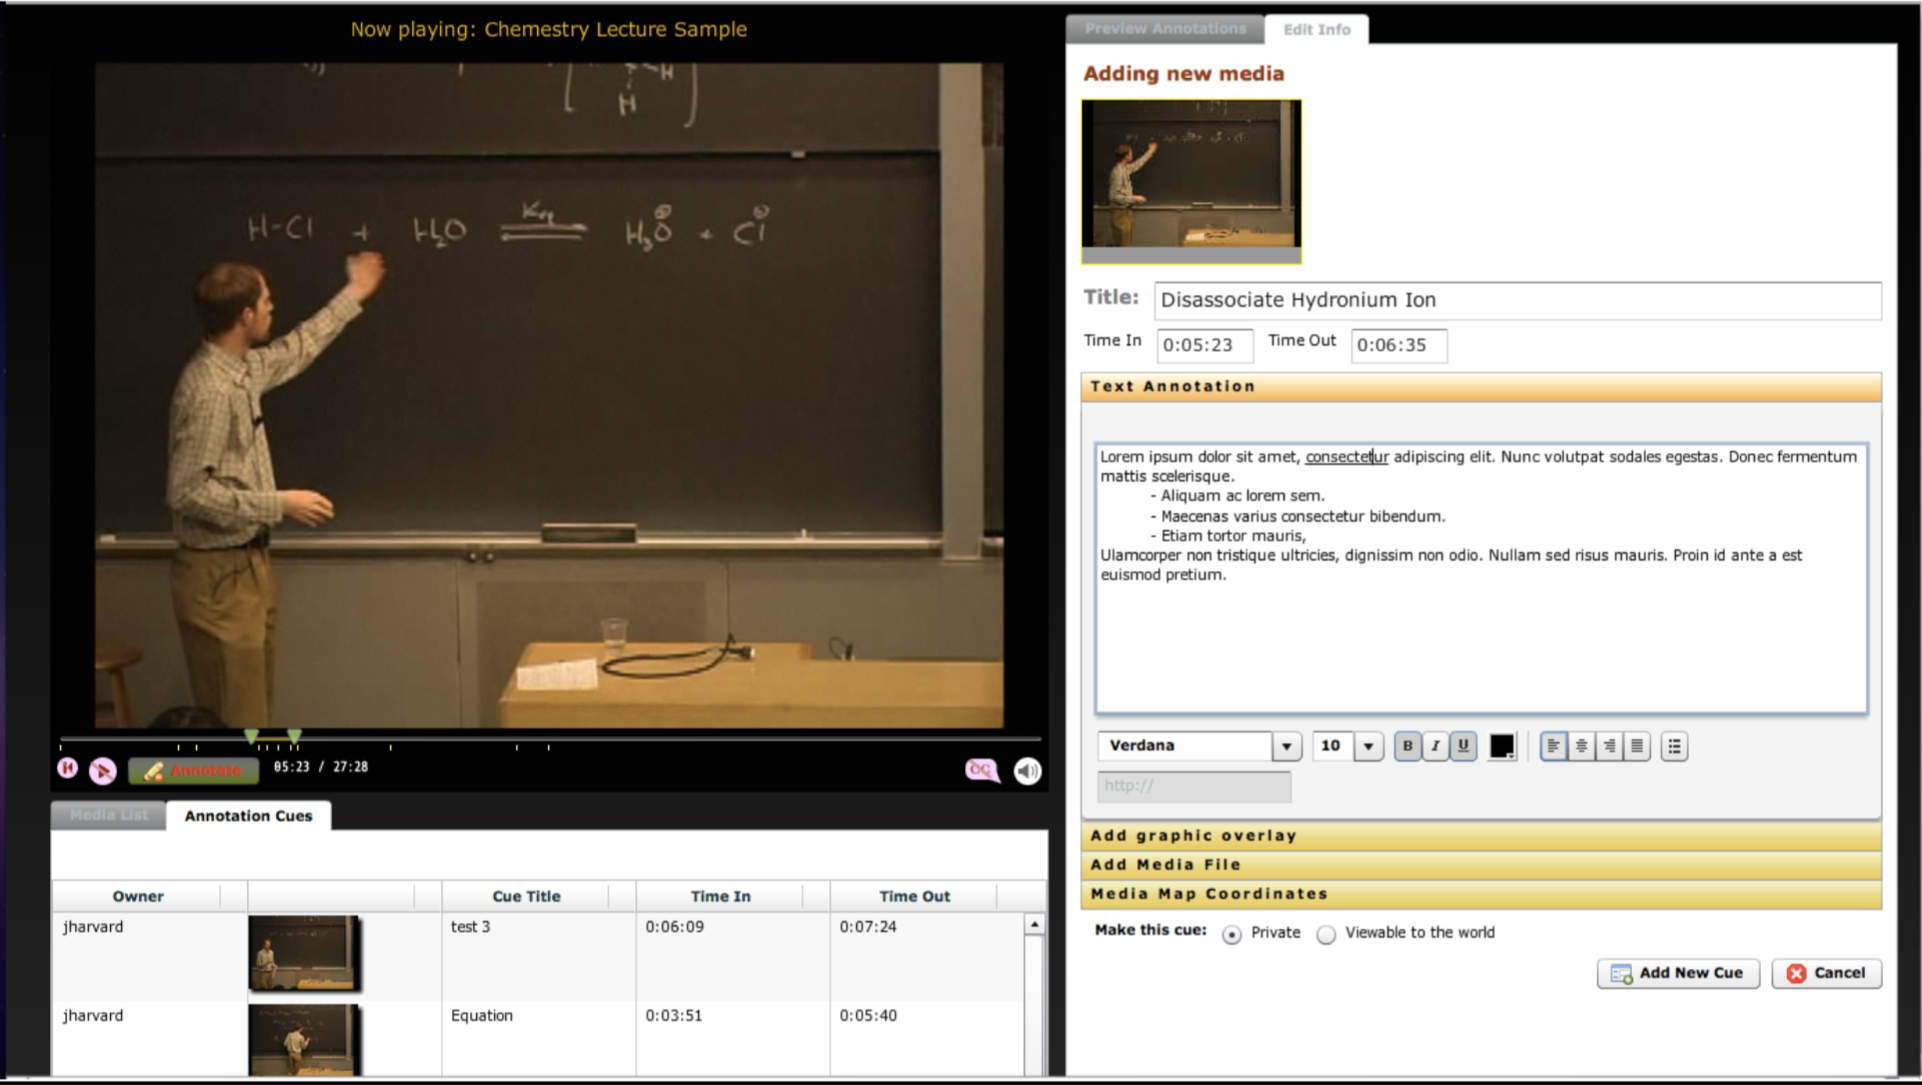
\includegraphics[width=1\textwidth]{gfx/mvat/mvat-annotation-edit-view.png}} \\
%{\centering

%\begin{figure}[htb]
%	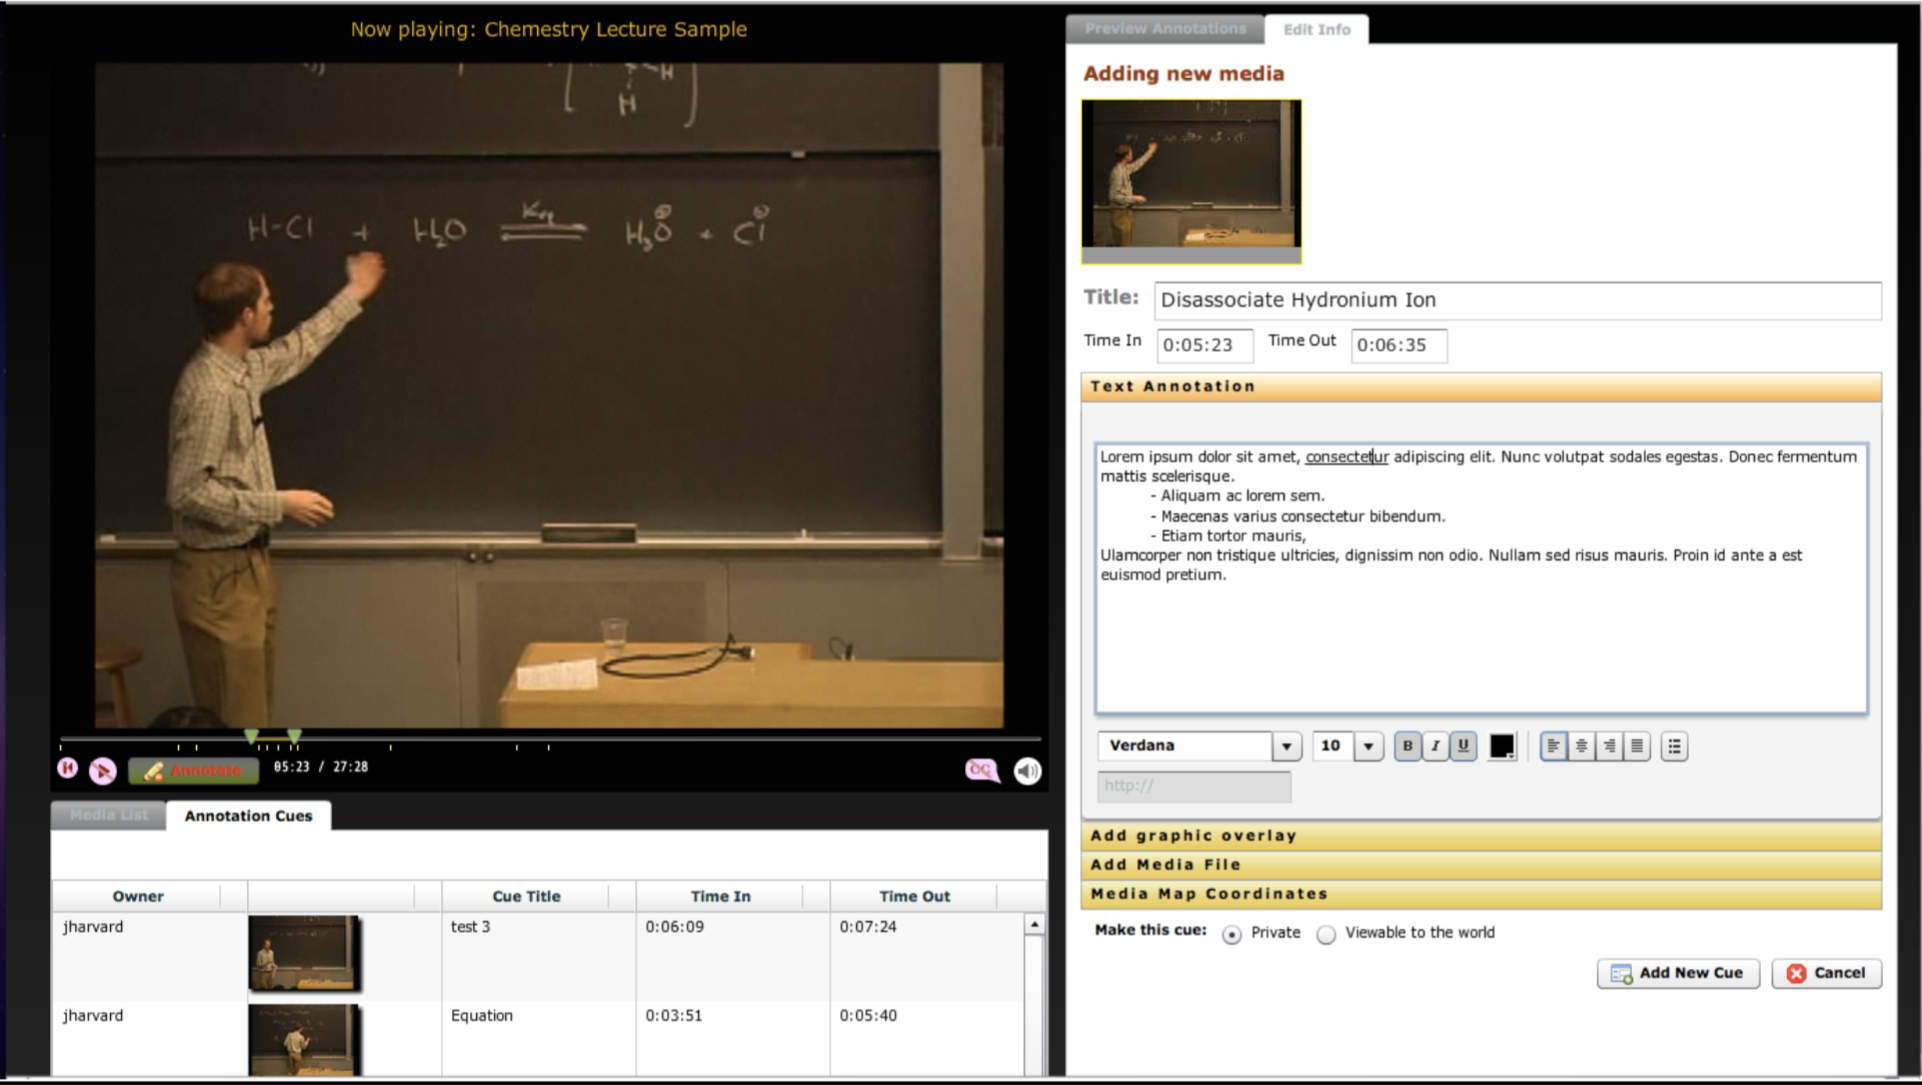
\includegraphics[width=\textwidth]{gfx/mvat/mvat-annotation-edit-view.png}
%	\caption{Figure example: \textit{(a)} example part one, \textit{(c)} example part two; \textit{(c)} example part three} 
%	\label{fig:mvat:example1}
%\end{figure} 
%\begin{figure}[htb]
%	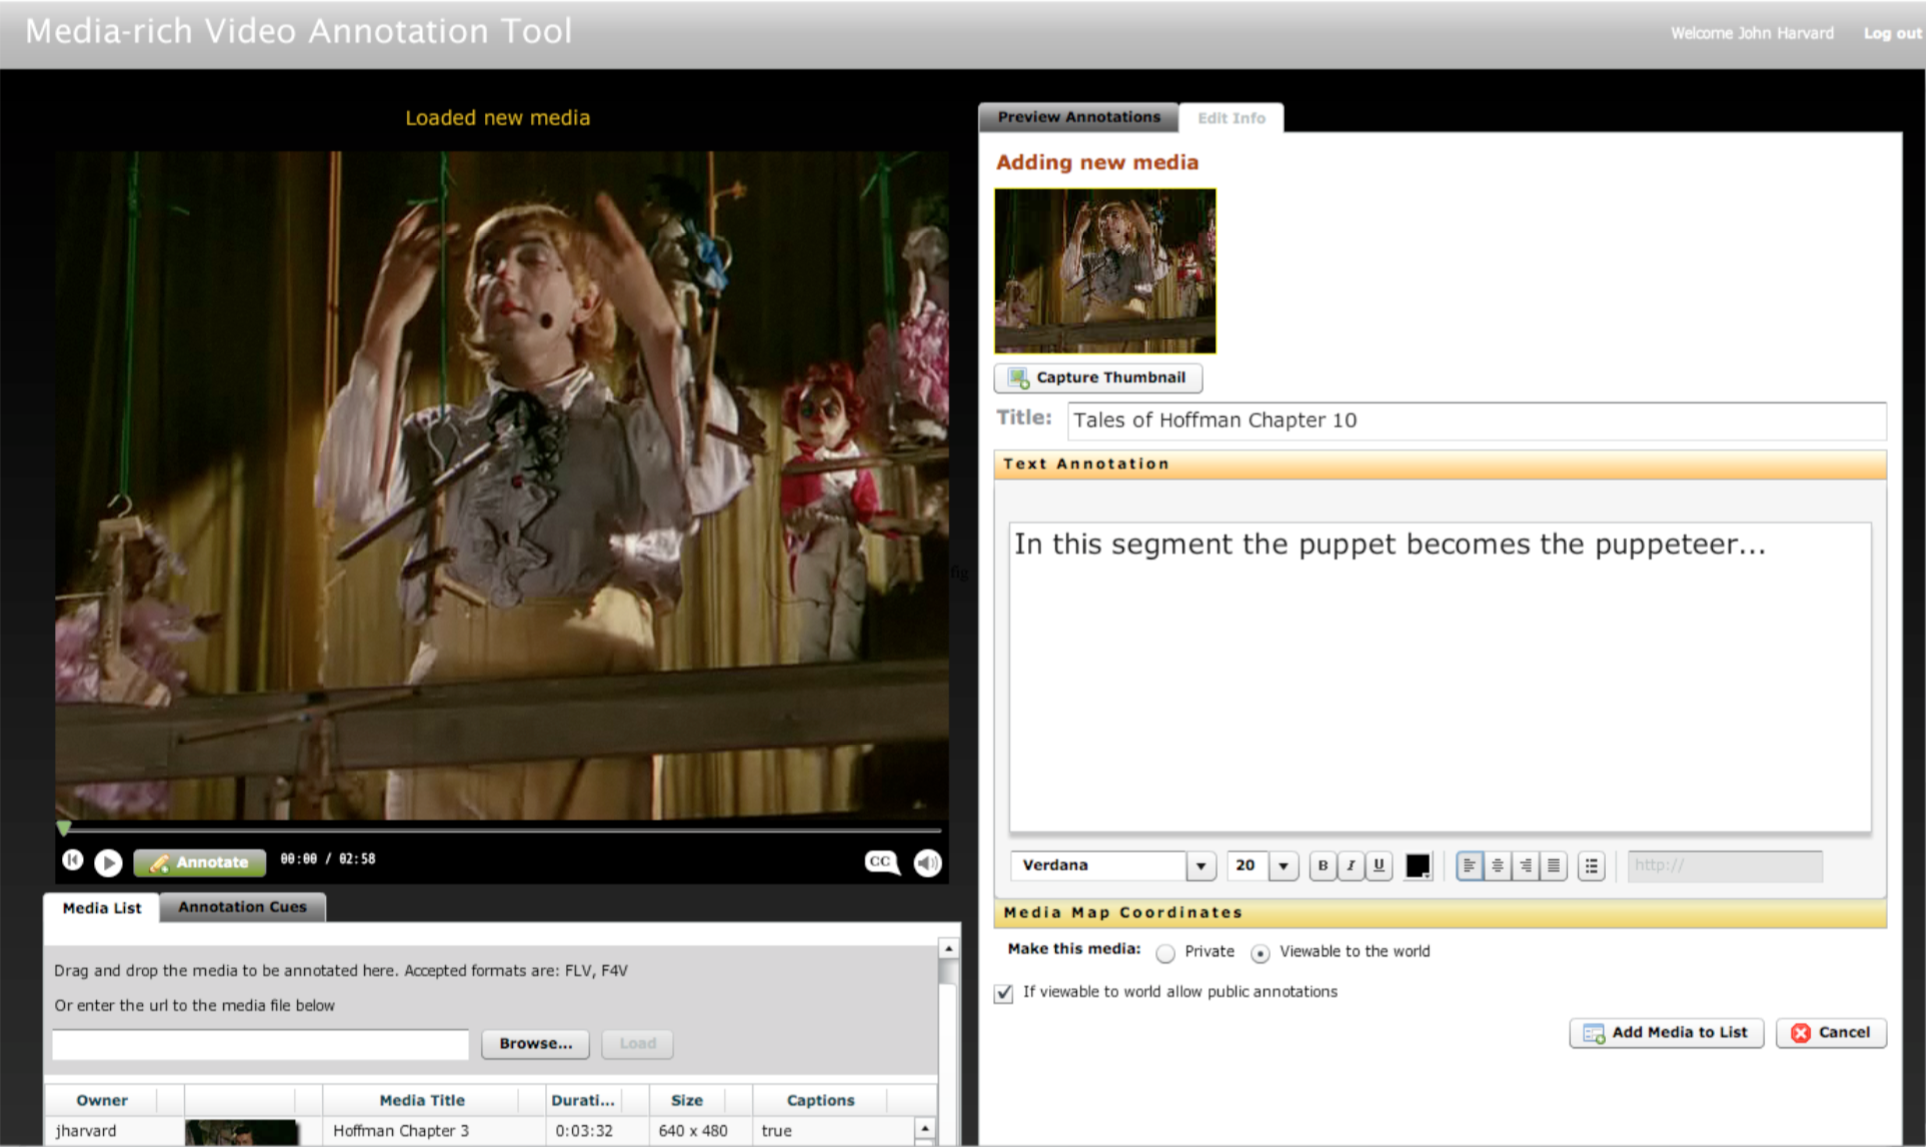
\includegraphics[width=\textwidth]{gfx/mvat/mvat-loading-video-adding-metadata.png}
%	\caption{Figure example: \textit{(a)} example part one, \textit{(c)} example part two; \textit{(c)} example part three} 
%	\label{fig:mvat:example2}
%\end{figure} 
%\begin{figure}[htb]
%	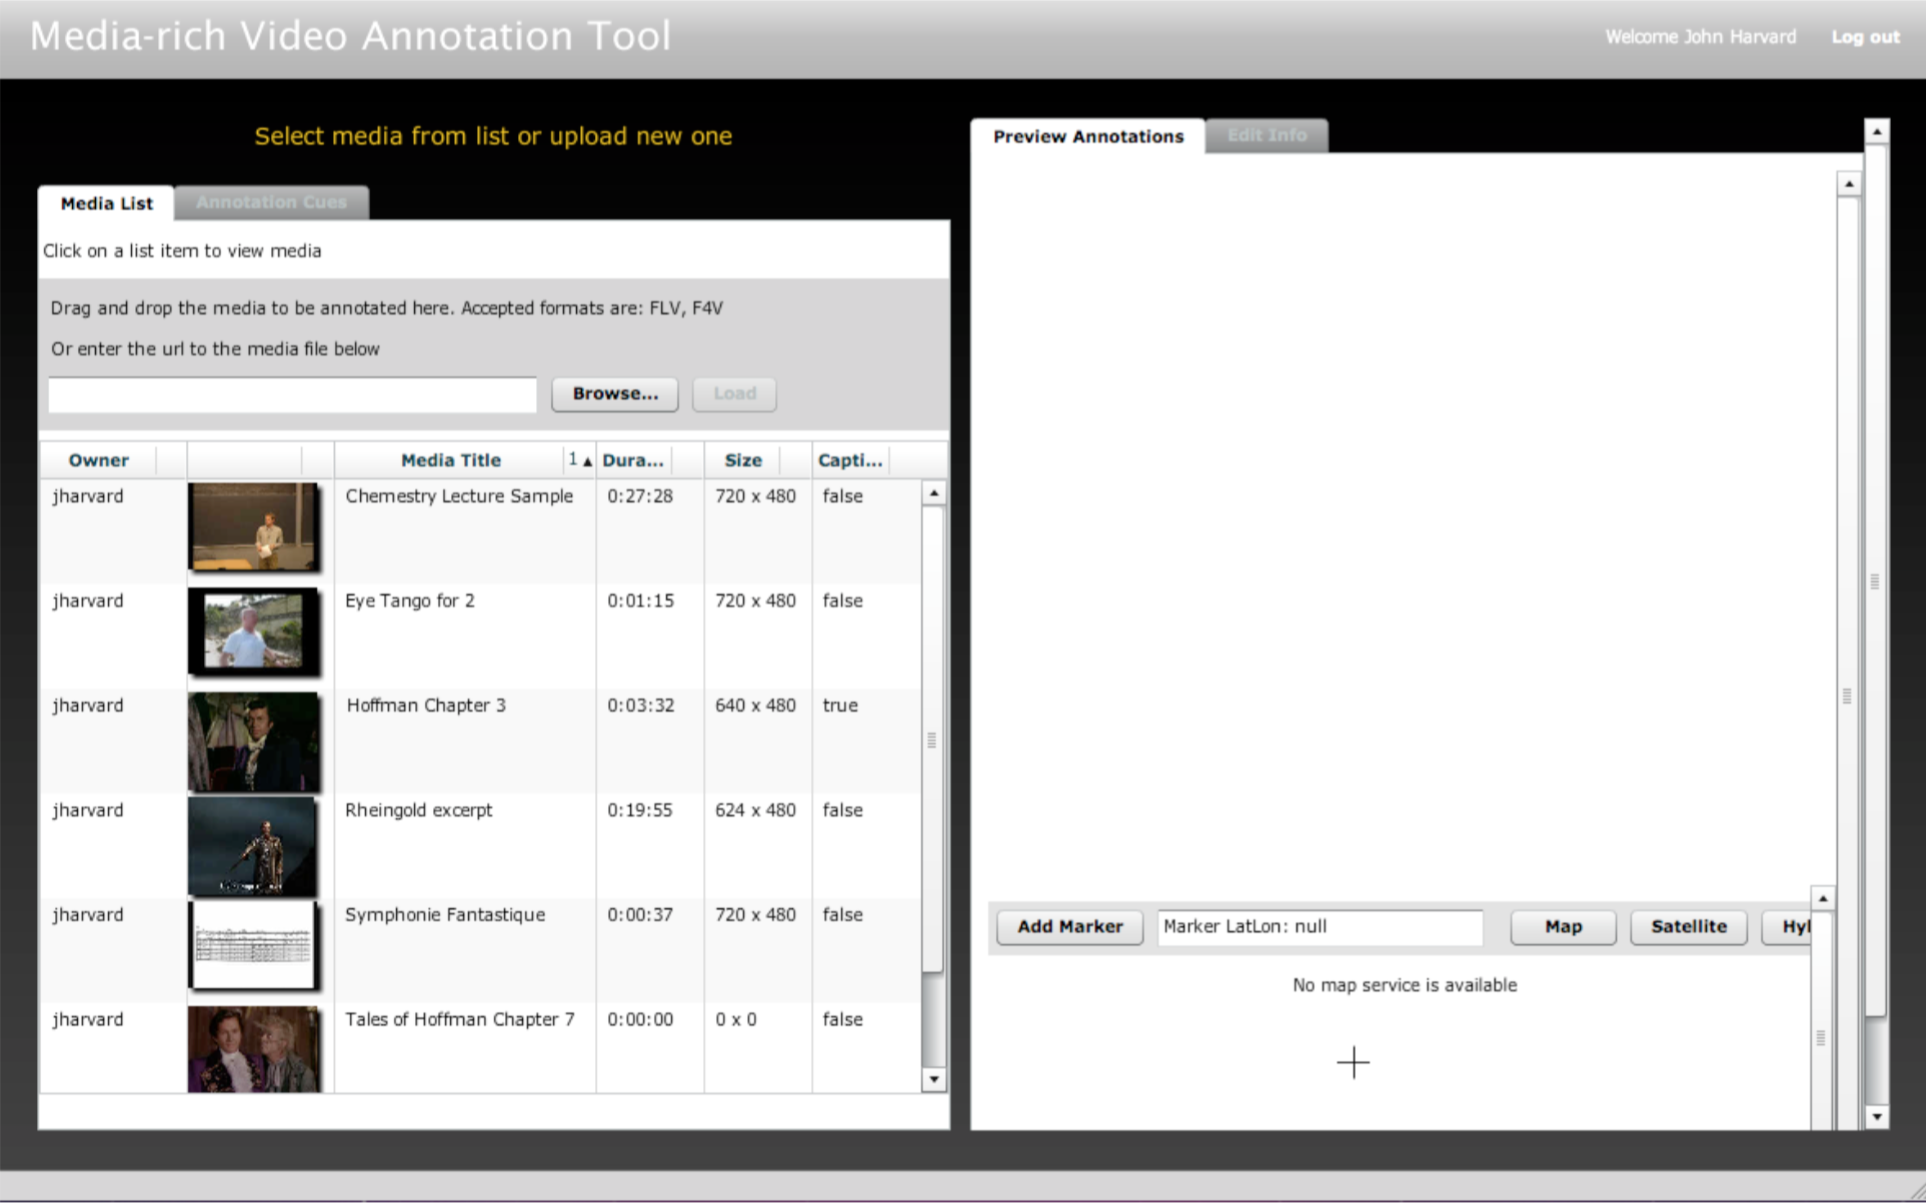
\includegraphics[width=\textwidth]{gfx/mvat/mvat-video-management}
%	\caption{Figure example: \textit{(a)} example part one, \textit{(c)} example part two; \textit{(c)} example part three}
%	\label{fig:mvat:example3}
%\end{figure}



%}

%\begin{figure}[htb]
%	
\includegraphics[width=\textwidth]{gfx/Clean-Thesis-Figure}
%	\caption{Figure example: \textit{(a)} example part one, \textit{(c)} example part two; \textit{(c)} example part three}
%	\label{fig:system:example1}
%\end{figure}
%
%\\ 
%%%%%%%%%%%{\centering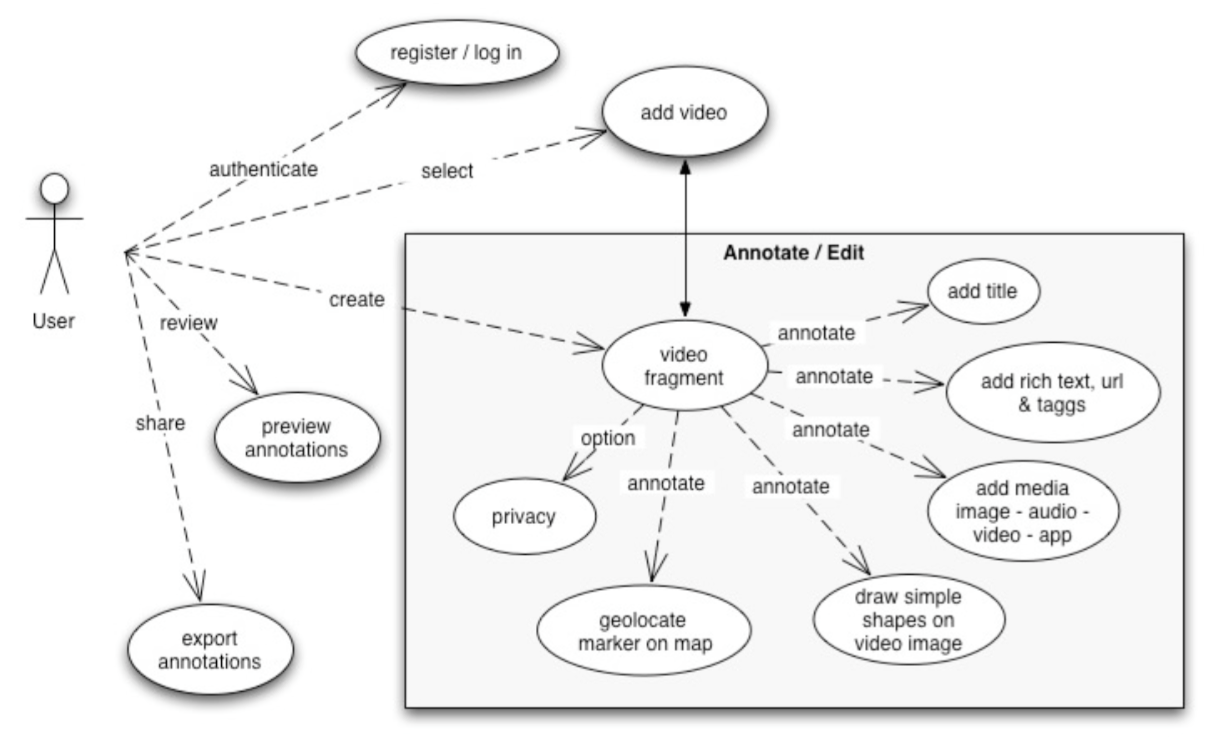
\includegraphics[width=1\textwidth]{gfx/mvat/mvat-core-use-case-diagram.png}} \\
%{\centering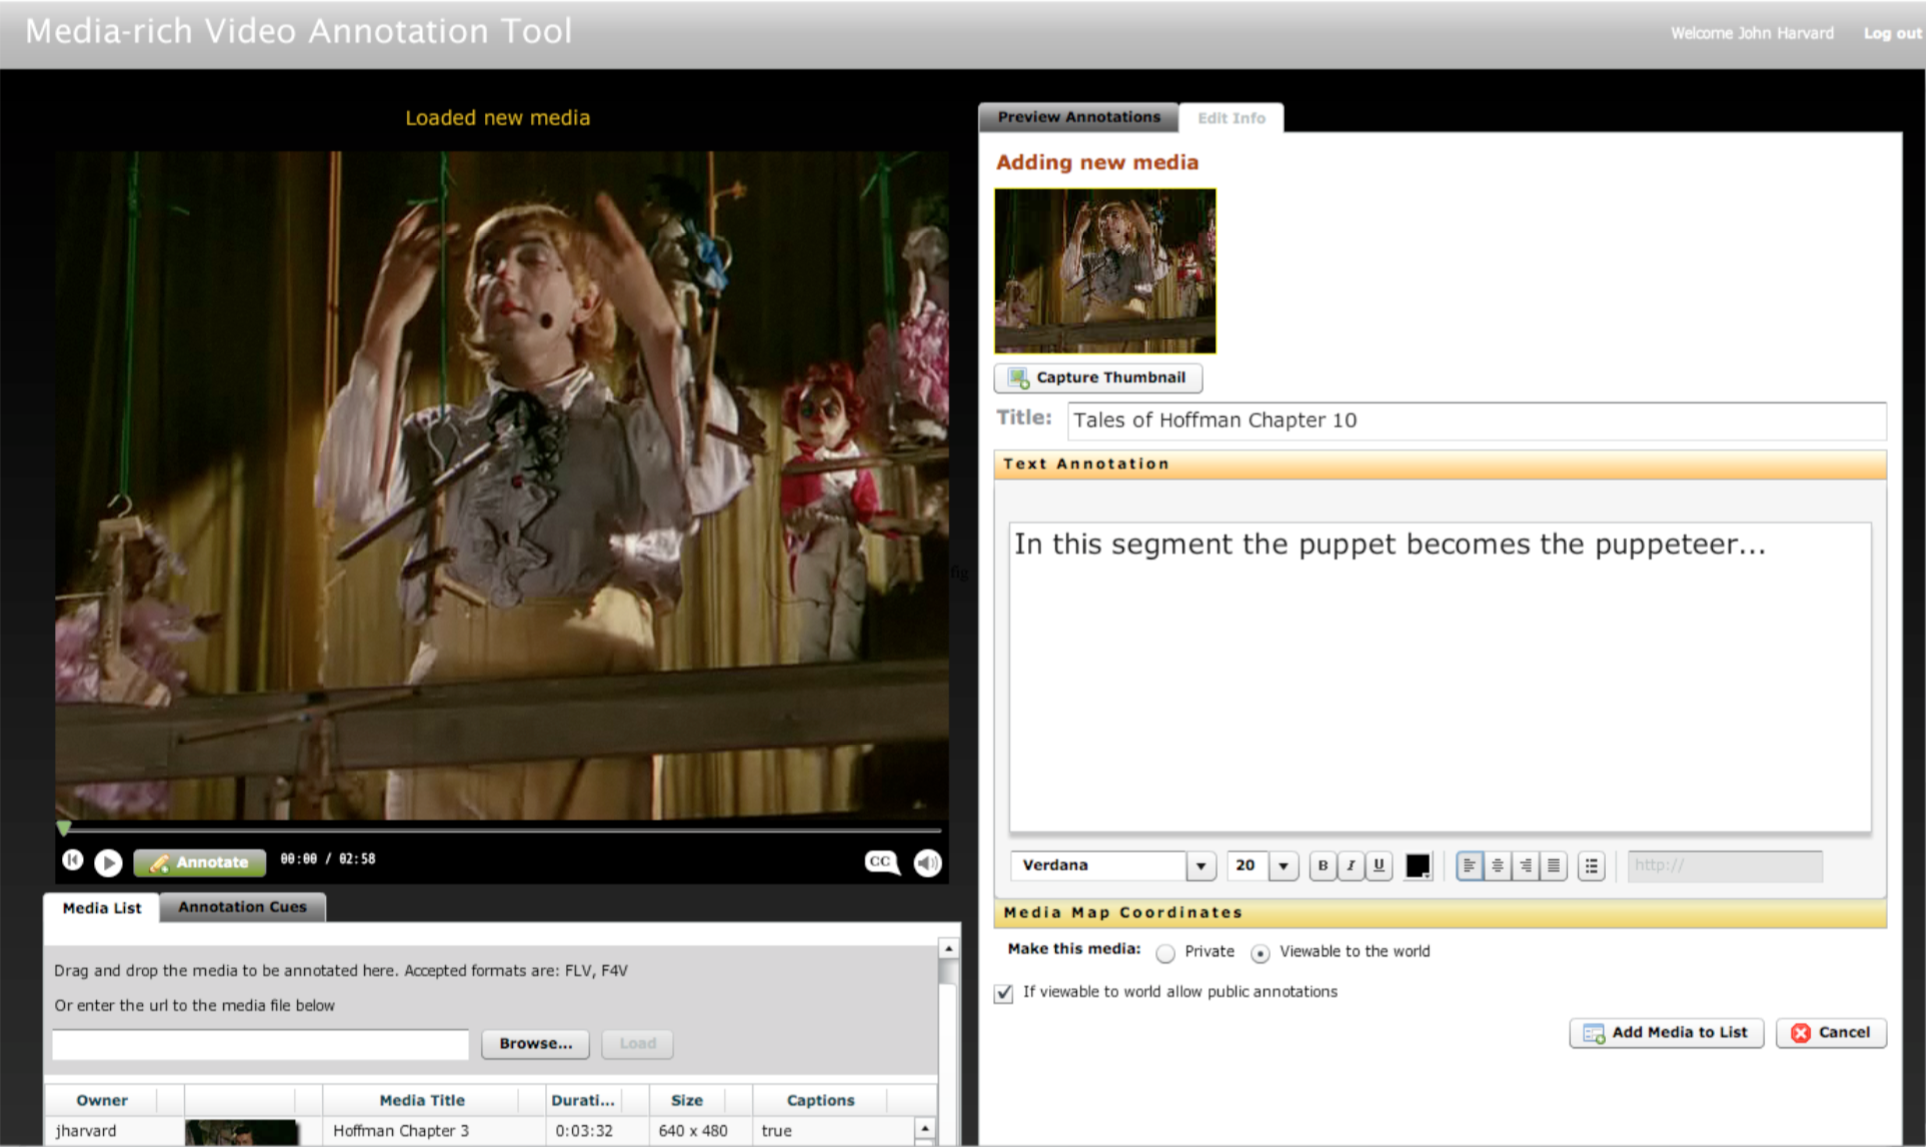
\includegraphics[width=1\textwidth]{gfx/mvat/mvat-loading-video-adding-metadata.png}} \\
%\\ 
%%%%%%%%%%%{\centering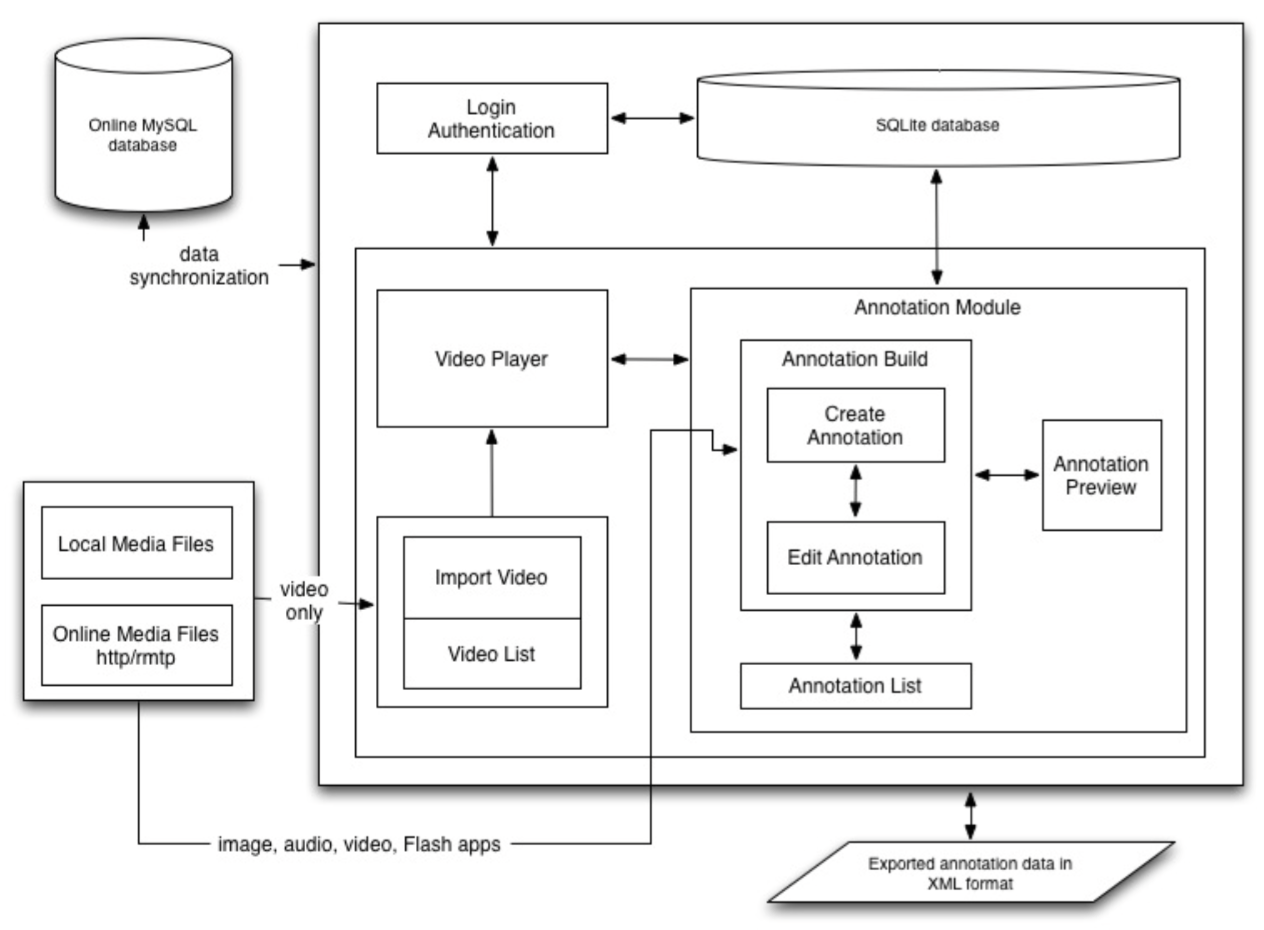
\includegraphics[width=1\textwidth]{gfx/mvat/mvat-system-architecture-overview.png}} \\
%%%%%%%%%%%{\centering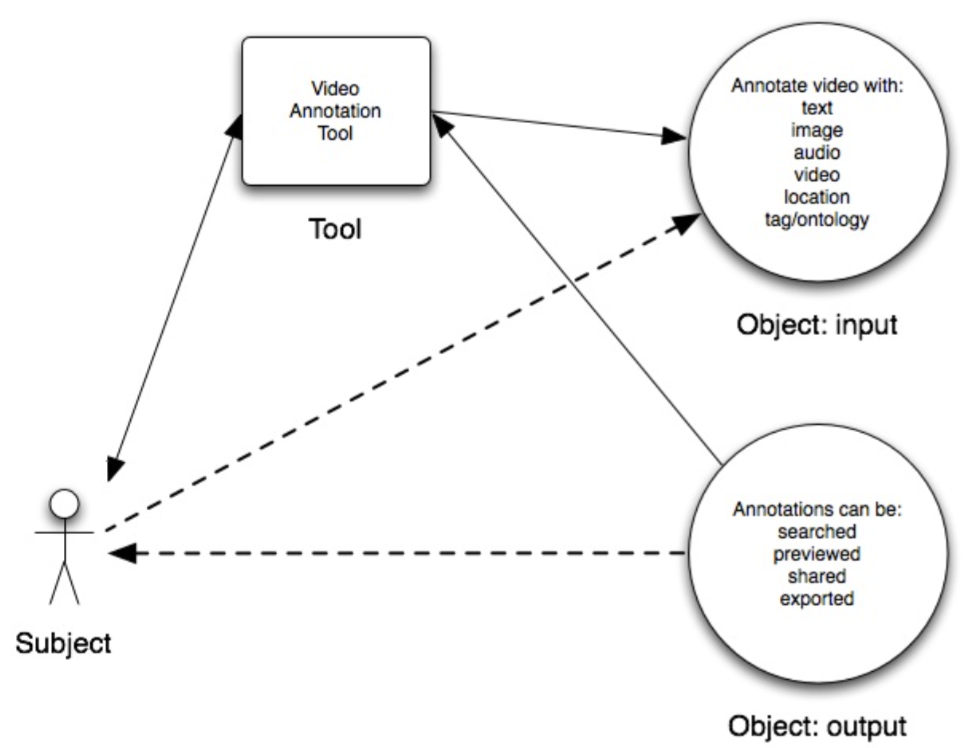
\includegraphics[width=1\textwidth]{gfx/mvat/mvat-use-case-diagram.png}} \\
%{\centering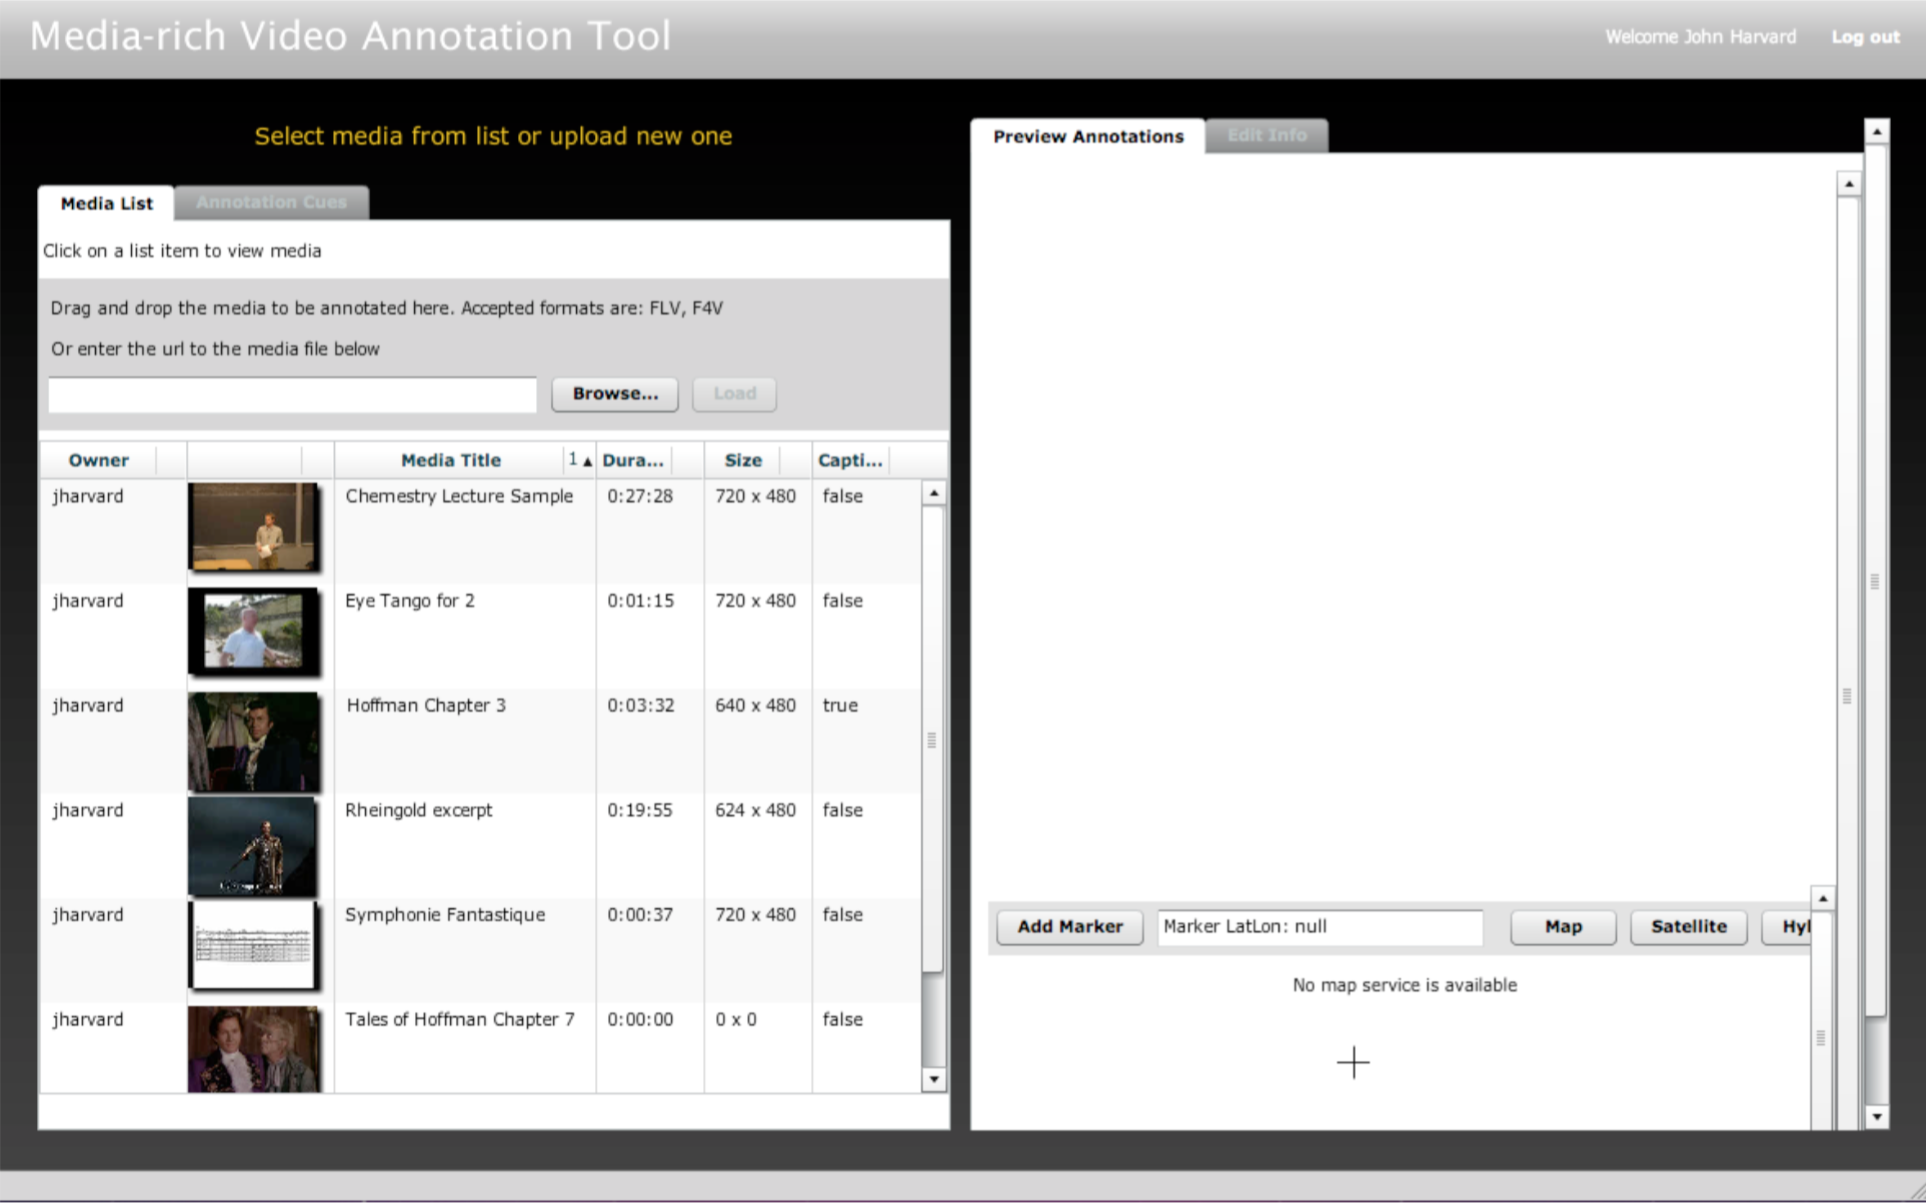
\includegraphics[width=1\textwidth]{gfx/mvat/mvat-video-management.png}} \\
%\\ 


%\href{http://www.people.fas.harvard.edu/~desenne/avac/}
%\href{https://forge.abcd.harvard.edu/gf/project/mvat/}
%\href{http://www.philipdesenne.com}
%\href{http://www.openvideoannotation.org/}

%\item \href{http://phx.corporate-ir.net/phoenix.zhtml?c=176060&p=irol-newsArticle&ID=2034369}{Amazon X-Ray}, by Amazon.com, Inc



\section{Amazon X-Ray}
\label{sec:priorwork:amazon-x-ray}
%\href{http://phx.corporate-ir.net/phoenix.zhtml?c=176060&p=irol-newsArticle&ID=2034369}{Amazon X-Ray}, by Amazon.com, Inc. \\
\textit{by Amazon.com, Inc.}

\begin{figure}[ht]
	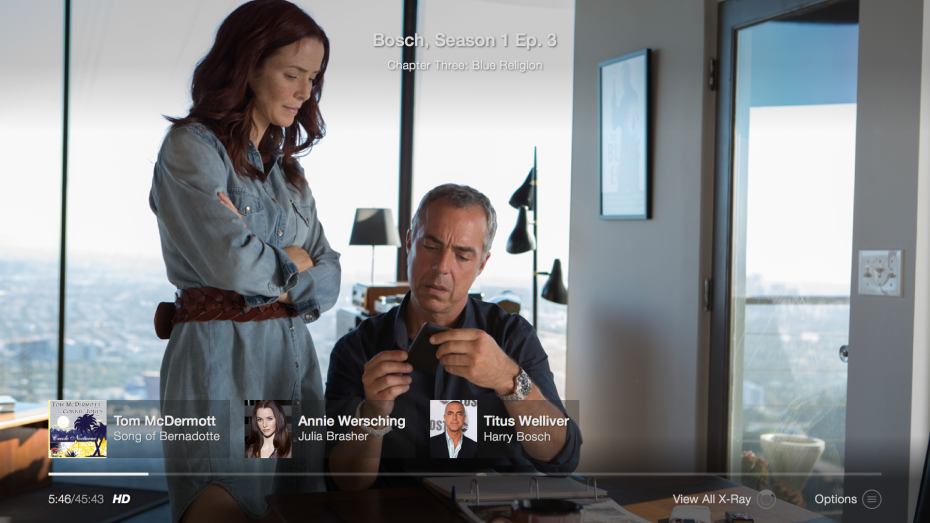
\includegraphics[width=\textwidth]{gfx/amazon-x-ray/pause-quick-view-930x523.png}
	\caption{\textit{(Amazon X-Ray)} pausing a video displays relevant annotations and links to \href{http://www.imdb.com}{IMDB}} 
	\label{fig:amazon-x-ray:paused-video-annotations}
\end{figure} 

\begin{figure}[ht]
	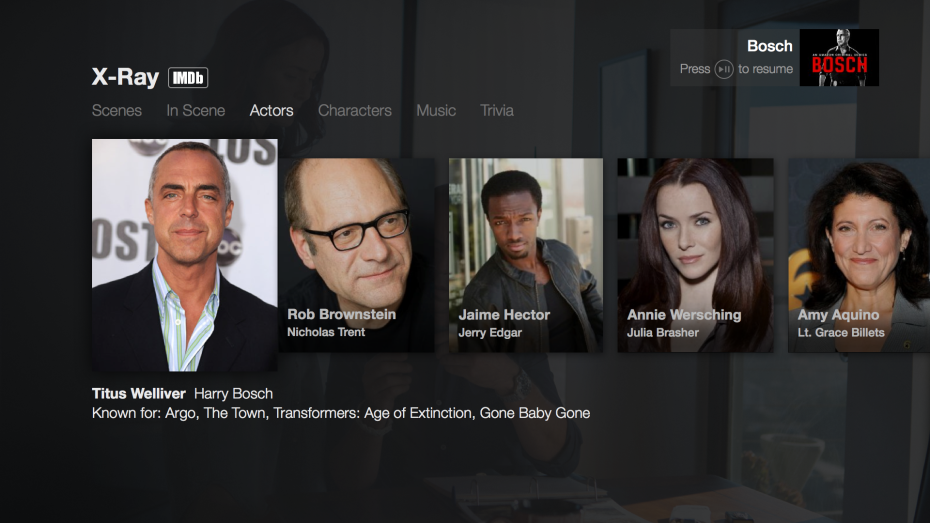
\includegraphics[width=\textwidth]{gfx/amazon-x-ray/xray-actors-930x523.png}
	\caption{\textit{(Amazon X-Ray)} displaying an annotation of all main actors in a film, linking to individual actor profiles on \href{http://www.imdb.com}{IMDB}} 
	\label{fig:amazon-x-ray:actors-listing}
\end{figure}

Amazon has developed a technology that is now being used in several of their video players, from HTML5 enabled web browsers, to portable devices such as the Kindle Fire, and to the Amazon Fire TV sticks. X-Ray presents a video overlay on top of a video as it is playing (or on some devices, when a video is paused) and shows relevant metadata such as the actors that are currently appearing onscreen (and links to their IMDB webpages), the director(s), links to artists whose music is currently playing, etc.  One of the motivating factors for the development of X-Ray for Amazon was to allow viewers to answer questions such as \textit{"Who's that guy?", "What's she been in?", or "What is that song?"} (see \url{http://www.businesswire.com/multimedia/home/20150413005383/en/}). 

The metadata that is used to power these real-time annotations comes from the \href{http://www.imdb.com/x-ray/}{Internet Movie Database}, which is an Amazon owned property.  Unfortunately there is not much in the way of technical details on the underlying technology or architecture of Amazon X-Ray, so it is difficult to find out how Amazon has created and implemented this technology, and how the metadata that powers the annotations is created (viewing an Amazon Prime hosted video in a web browser, for example, show you these annotations when you mouseover the player windown, and the annotations change as characters move in and out of screen, when a new song begins and ends, etc.).

For more information on Amazon X-Ray, see:
\begin{itemize}[noitemsep,leftmargin=*]
\item \url{http://www.imdb.com/x-ray/}
\item \url{http://www.businesswire.com/multimedia/home/20150413005383/en/}
\item \url{http://phx.corporate-ir.net/phoenix.zhtml?c=176060&p=irol-newsArticle&ID=2034369}
\item \url{http://www.engadget.com/2012/09/06/amazon-announces-x-ray-for-movies-a-kindle-feature-that-uses-im/}
\item \url{http://venturebeat.com/2015/04/13/amazons-x-ray-arrives-for-fire-tv-and-fire-tv-stick-bringing-context-to-instant-video-on-the-big-screen/}
\item \url{http://www.wired.com/2015/04/amazon-xray-fire-tv/}
\item \url{http://gizmodo.com/5941067/amazons-x-ray-for-movies-knows-what-youre-watchingand-whos-in-it}
\end{itemize}


%\end{enumerate}


%\section{Prior Work Section 1}
%\label{sec:priorwork:sec1}

%\section{Prior Work Section 2}
%\label{sec:priorwork:sec2}

%\section{Prior Work Section 3}
%\label{sec:priorwork:sec3}


\section{Conclusion}
\label{sec:priorwork:conclusion}

There has been some very interesting and promising scholarly work done in the area of video annotations previously, but this thesis project has several unique aspects that it attempts to add and extend off of such prior work to make this project novel. Prior work does not appear to have focused too much on the search aspects of annotations that area created or the discoverability of videos that users might not have otherwise ever seen or known about were the annotations not present.  Social sharing aspects of prior work in the area of video annoation seems to be a missing aspect of much prior work as well.  A large part of the impetus for this project is the acknowledgement that the user in posession of a recording may themselves not know enough to properly annotate the video, but knows others (in this particular case, family members, but the same logic could easily apply to friends, colleagues, classmates, etc.) that would be able to add correct annotations.

%\Blindtext[2][1]
